% Options for packages loaded elsewhere
\PassOptionsToPackage{unicode}{hyperref}
\PassOptionsToPackage{hyphens}{url}
\PassOptionsToPackage{dvipsnames,svgnames*,x11names*}{xcolor}
%
\documentclass[
  spanish,
  a4paper,
  openany]{book}
\usepackage{amsmath,amssymb}
\usepackage[]{bookman}
\usepackage{ifxetex,ifluatex}
\ifnum 0\ifxetex 1\fi\ifluatex 1\fi=0 % if pdftex
  \usepackage[T1]{fontenc}
  \usepackage[utf8]{inputenc}
  \usepackage{textcomp} % provide euro and other symbols
\else % if luatex or xetex
  \usepackage{unicode-math}
  \defaultfontfeatures{Scale=MatchLowercase}
  \defaultfontfeatures[\rmfamily]{Ligatures=TeX,Scale=1}
\fi
% Use upquote if available, for straight quotes in verbatim environments
\IfFileExists{upquote.sty}{\usepackage{upquote}}{}
\IfFileExists{microtype.sty}{% use microtype if available
  \usepackage[]{microtype}
  \UseMicrotypeSet[protrusion]{basicmath} % disable protrusion for tt fonts
}{}
\makeatletter
\@ifundefined{KOMAClassName}{% if non-KOMA class
  \IfFileExists{parskip.sty}{%
    \usepackage{parskip}
  }{% else
    \setlength{\parindent}{0pt}
    \setlength{\parskip}{6pt plus 2pt minus 1pt}}
}{% if KOMA class
  \KOMAoptions{parskip=half}}
\makeatother
\usepackage{xcolor}
\IfFileExists{xurl.sty}{\usepackage{xurl}}{} % add URL line breaks if available
\IfFileExists{bookmark.sty}{\usepackage{bookmark}}{\usepackage{hyperref}}
\hypersetup{
  pdftitle={Manual de privacidad y seguridad en internet},
  pdfauthor={Diego Chiquero Mena},
  pdflang={es},
  pdfkeywords={seguridad,privacidad, ciberdelitos, ciberdelincuentes,internet},
  colorlinks=true,
  linkcolor=blue,
  filecolor=Maroon,
  citecolor=Blue,
  urlcolor=Blue,
  pdfcreator={LaTeX via pandoc}}
\urlstyle{same} % disable monospaced font for URLs
\usepackage[top=1in,bottom=1in,right=1in,left=1in]{geometry}
\usepackage{longtable,booktabs,array}
\usepackage{calc} % for calculating minipage widths
% Correct order of tables after \paragraph or \subparagraph
\usepackage{etoolbox}
\makeatletter
\patchcmd\longtable{\par}{\if@noskipsec\mbox{}\fi\par}{}{}
\makeatother
% Allow footnotes in longtable head/foot
\IfFileExists{footnotehyper.sty}{\usepackage{footnotehyper}}{\usepackage{footnote}}
\makesavenoteenv{longtable}
\usepackage{graphicx}
\makeatletter
\def\maxwidth{\ifdim\Gin@nat@width>\linewidth\linewidth\else\Gin@nat@width\fi}
\def\maxheight{\ifdim\Gin@nat@height>\textheight\textheight\else\Gin@nat@height\fi}
\makeatother
% Scale images if necessary, so that they will not overflow the page
% margins by default, and it is still possible to overwrite the defaults
% using explicit options in \includegraphics[width, height, ...]{}
\setkeys{Gin}{width=\maxwidth,height=\maxheight,keepaspectratio}
% Set default figure placement to htbp
\makeatletter
\def\fps@figure{htbp}
\makeatother
\setlength{\emergencystretch}{3em} % prevent overfull lines
\providecommand{\tightlist}{%
  \setlength{\itemsep}{0pt}\setlength{\parskip}{0pt}}
\setcounter{secnumdepth}{5}
\usepackage{graphicx}
\usepackage{fancyhdr}
\pagestyle{plain}
\renewcommand{\headrulewidth}{0.2pt}
\usepackage{floatpag}
\floatpagestyle{empty}
\ifxetex
  % Load polyglossia as late as possible: uses bidi with RTL langages (e.g. Hebrew, Arabic)
  \usepackage{polyglossia}
  \setmainlanguage[]{spanish}
\else
  \usepackage[main=spanish]{babel}
% get rid of language-specific shorthands (see #6817):
\let\LanguageShortHands\languageshorthands
\def\languageshorthands#1{}
\fi
\ifluatex
  \usepackage{selnolig}  % disable illegal ligatures
\fi
\usepackage[]{natbib}
\bibliographystyle{apalike}

\title{Manual de privacidad y seguridad en internet}
\author{Diego Chiquero Mena}
\date{30 marzo 2021}

\begin{document}
\maketitle

\thispagestyle{empty}
\begin{center}
\noindent\makebox[\textwidth]{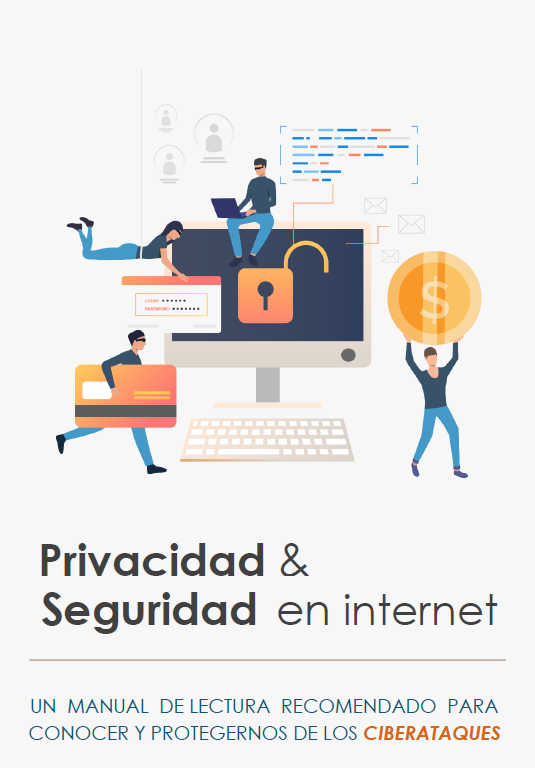
\includegraphics[width=\paperwidth]{images/cover.png}}
%\makebox[\textwidth]{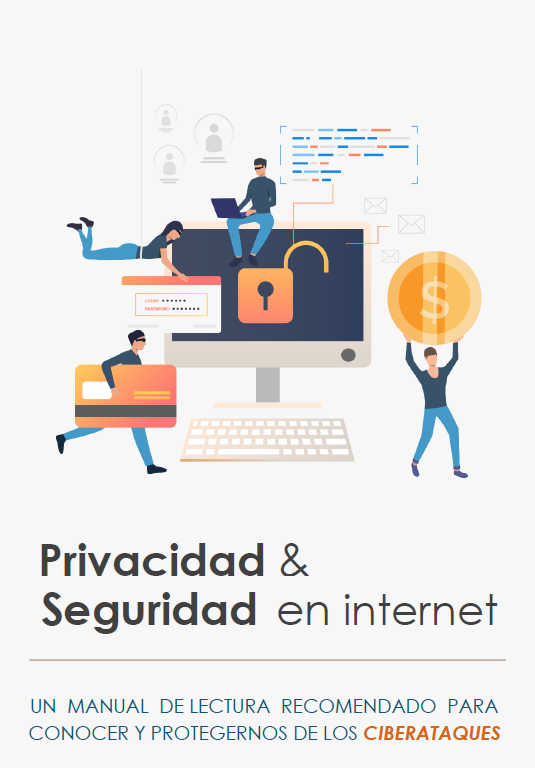
\includegraphics[width=\paperwidth]{images/cover.png}}
\end{center}
\fontsize{14}{16}
%\fontseries{b}
\selectfont





{
\hypersetup{linkcolor=}
\setcounter{tocdepth}{3}
\tableofcontents
}
\hypertarget{pruxf3logo}{%
\chapter*{Prólogo}\label{pruxf3logo}}
\addcontentsline{toc}{chapter}{Prólogo}

Este manual aglutina de manera filtrada y tamizada una amplia y detallada parte del conocimiento e información de relevancia que puedes encontrar en la web sobre privacidad y seguridad en internet, de forma ordenada y estructura. Además encontrarás en la bibliografía todas las fuentes que han hecho posible la elaboración y documentación de este manual, para que puedas contrastar por ti mismo dichas fuentes.

Entenderás las diferencias entre los conceptos de privacidad y seguridad en internet, para que de este modo puedas hacer una buena configuración y uso de éstas.

Aprenderás buenas prácticas en la gestión de la privacidad, así como la manera más adecuada de gestionar la seguridad tanto en los equipos (PC, tables, smartphones, etc.), como en la red de datos.

Conocerás las principales amenazas que existen en el uso de las tecnologías y el mundo digital.

Y por último, pero no por ello menos importante, se abordarán otros conceptos relacionados con los ciberdelitos, la huella digital, la importancia de ser selectivos con la información online y otros aspectos más.

Para concluir, también encontrarás a lo largo del manual multitud de enlaces que te llevarán a más información ampliada sobre las temáticas, así como una extensa lista de recursos y herramientas para que puedas llevar tu privacidad y seguridad en internet al siguiente nivel.

Si quieres contribuir y ayudar a nutrir de más contenido de valor este manual, por favor, no lo dudes y ponte en contacto conmigo, estaré encantado que colaboremos. Encontrarás mis datos de contacto en el siguiente apartado \emph{sobre el autor}.

Este manual está disponible en el repositorio Github: \href{https://github.com/diegochiquero/manual-de-privacidad-y-seguridad-en-internet}{diegochiquero/manual-de-privacidad-y-seguridad-en-internet}. Y ha sido escrito en \href{http://rmarkdown.rstudio.com}{R-Markdown} empleando el paquete \href{https://bookdown.org/}{\texttt{bookdown}} cuya guia encontrarás en \citep{R-bookdown}.

Imagen portada \citep{freepik}

Esta obra está bajo la \href{https://creativecommons.org/licenses/by-nc-sa/4.0/deed.es}{licencia Creative Commons Atribución-NoComercial-CompartirIgual 4.0 Internacional}.

\begin{flushleft}
\includegraphics{images/by-nc-sa-88x31} \end{flushleft}

\hypertarget{autor}{%
\chapter*{Sobre el autor}\label{autor}}
\addcontentsline{toc}{chapter}{Sobre el autor}

\begin{flushleft}
\includegraphics[width=0.25\linewidth]{images/diego-chiquero-2020-profile} \end{flushleft}

Hola, mi nombre en Diego.

Y lo primero que me gustaría hacer, es agradecerte que hayas decidido leer este manual. Ya que éste hecho, hace que las horas de dedicación, esfuerzo, documentación y contrastación de fuentes hayan merecido la pena.

El propósito de este manual es hacerte consciente de los peligros de navegar por internet, de lo vulnerable y expuesto que puedes llegar a estar en el uso de las tecnologías y a su vez dotarte de conocimientos, consejos y herramientas para poder hacer una buena gestión de la web de manera segura y privada.

De formación académica Técnico superior en desarrollo de aplicaciones web.
Para concluir y a modo de breve presentación, haré referencia a mi extracto de Linkedin:

\begin{quote}
Apasionado de las tecnologías, el espíritu empresarial y la programación.

Plenamente convencido que las competencias transversales pueden marcan la diferencia, que el derecho nos asiste a todos y que un mundo mejor es posible.

En continuo proceso de crecimiento personal y profesional.
\end{quote}

Diego Chiquero Mena

Puedes contactar conmigo en \href{mailto:chiquerodiego@yahoo.es}{\nolinkurl{chiquerodiego@yahoo.es}}

Más sobre mí \href{https://about.me/diegochiquero}{Diego Chiquero Mena}

\hypertarget{privacidad-y-seguridad-en-internet}{%
\chapter{Privacidad y Seguridad en Internet}\label{privacidad-y-seguridad-en-internet}}

\hypertarget{introducciuxf3n}{%
\section{Introducción}\label{introducciuxf3n}}

En estos últimos años hemos podido ver como la evolución de las IT (Tecnologías de la información) y el paso de la Web1.0. a la Web 2.0., nos ha permitido a muchos de nosotros como usuarios interactuar los unos con los otros subiendo y compartiendo todo tipo de contenidos. La aparición de las Redes sociales ha traído con ellas, la posibilidad de publicar fotos, videos, información, comentarios, reseñas, etc. a través de cualquier dispositivo, ya sea un PC, tablet o smartphone. Y no solo eso, sino que además, también nos ha abierto un amplio abanico de posibilidades con las que podemos gestionar cuentas bancarias, hacer compras online, trámites telemáticos y un sinfín de gestiones que hasta hace tan solo unos años atrás eran difíciles de imaginar.

Como consecuencia de ello, el enorme conglomerado de información sensible que se encuentra disponible en internet, hace que nosotros como usuarios estemos en el punto de mira de ciberdelincuentes y expuestos a todo tipo de ciberataques. En esta línea, este manual contribuye a enseñarte, aconsejarte y proveerte de herramientas necesarias para prevenir, evitar y paliar en la medida de lo posible todos los riesgos y peligros a los que estamos expuestos en nuestro uso diario de las tecnologías.

Por lo tanto, en lo sucesivo iras viendo el porqué de la importancia de velar de manera activa por tu privacidad y seguridad en internet haciendo una buena gestión de éstas. También te ayudará a conocer y reconocer la amplia lista de ciberdelitos que actualmente están más extendidos.

En estás \href{https://oedi.es/estadisticas/}{estadísticas} públicadas por el Observatorio Español de Delitos informáticos \citep{oedi} puedes ver el porqué de cuidar tu privacidad y seguridad en internet. En ellas se expone una exhaustiva lista de ciberdelitos y sus recurrencias cronológicas.

\hypertarget{privacidad}{%
\section{Privacidad}\label{privacidad}}

La privacidad es aquello que se lleva a cabo en un ámbito reservado; en Internet podría entenderse como el control que ejercemos sobre nuestra información para limitar la cantidad de personas autorizadas a verla, así como la cantidad de contenido expuesto. Esto incluye datos personales, fotografías, documentos, etc.

Internet es una herramienta que nos permite la interacción entre dos o más personas. Siendo ejemplo de los anteriores sitios como Facebook y Twitter, Redes Sociales en donde las personas pueden compartir públicamente opiniones, noticias, sentimientos, ideas, fotografías, videos, etc. Por ello es necesario considerar que Internet es un espacio abierto al mundo, por lo tanto, cualquier acción que se haga va a tener un impacto global y permanente. Por ejemplo, imagina una publicación de la cual puedas arrepentirte (como una fotografía u opinión) no solo podrá ser vista por millones de usuarios , sino que también será prácticamente imposible de borrar completamente de la red .

También puede resultar peligroso publicar datos que puedan identificarte, como la dirección, teléfonos, lugar de estudio o trabajo, días de vacaciones, etc. Esto puede resultar todavía más complicado si posees una gran lista de amigos a los que no conoces personalmente.

Por todo lo que se ha mencionado en éstas últimas líneas, es de suma importancia que antes de publicar algo, pienses en las consecuencias que puede conllevar divulgar información sensible en sitios públicos y de los cuales no siempre se tiene un control directo \citep{privacidad}.

\hypertarget{seguridad}{%
\section{Seguridad}\label{seguridad}}

La seguridad en internet son todas aquellas precauciones que son tomadas para proteger todos los dispositivos informáticos, así como la red de internet que pueden ser afectados por delincuentes cibernéticos. Además de ser una rama de la seguridad informática que se dedica a identificar y prevenir todas las amenazas que afectan a la red de redes, siendo una de las herramientas más conocidas los antivirus \citep{seguridad}.

Entre los peligros más habituales de no hacer un buen uso de la seguridad en la red, nos encontramos, robo de datos bancarios o personales, virus informáticos, phishing, spam, etc. Pero estos no son losúnicos riesgos que asechan en internet, como verás más adelante.

\hypertarget{rgpd-reglamento-general-de-protecciuxf3n-de-datos}{%
\section{RGPD (Reglamento general de protección de datos)}\label{rgpd-reglamento-general-de-protecciuxf3n-de-datos}}

El Reglamento General de Protección de Datos (RGPD) es el reglamento europeo relativo a la protección de las personas físicas en lo que respecta al tratamiento de sus datos personales y a la libre circulación de estos datos. Entró en vigor el 25 de mayo de 2016 y fue de aplicación el 25 de mayo de 2018, dos años durante los cuales las empresas, las organizaciones, los organismos y las instituciones han debido ir adaptándose para su cumplimiento. Es una normativa a nivel de la Unión Europea, por lo que cualquier empresa de la unión, o aquellas empresas que tengan negocios en la Unión Europea, que manejen información personal de cualquier tipo deberán acogerse a la misma \citep{WIKI-rgpd}.

En el pasado el uso de datos eran obtenido por omisión, en estos momentos para estar seguros de cumplir con el RGPD se ha de obtener el consentimiento inequívoco o expreso por parte del usuario.

Paralela a la RGPD europea existe una a nivel de España llamada Ley orgánica de protección de datos y garantía de los derechos digitales, recogida en el BOE \href{https://www.boe.es/buscar/doc.php?id=BOE-A-2018-16673}{Boletín Oficial del Estado} y cuyo objeto es también garantizar y proteger las libertades públicas y los derechos fundamentales de las personas físicas y en especial, su honor e integridad personal y familiar.

Entre los aspectos más significativos del RGPD cabe destacar los siguientes:

\begin{itemize}
\item
  Derecho a la portabilidad de los datos: Te da el derecho de solicitar al responsable de tus datos el traspaso de éstos a otra entidad o responsable. Un ejemplo claro es la conocida portabilidad en el mundo de la telefonía que hacen que tus datos puedas ser cedidos de una compañía a otra.
\item
  Derecho a la supresión: Es una versión mejorada de la solicitud de cancelación o eliminación de tus datos.
\item
  Derecho al olvido: Te da derecho a solicitar al responsable de tus datos la supresión o eliminación de éstos pero con un enfoque más estrecho con el ámbito digital. Desde el servicio ofrecido por \href{https://www.aepd.es/es/areas-de-actuacion/internet-y-redes-sociales/derecho-al-olvido}{AEPD} pudes acceder a los enlaces donde solicitar el derecho al olvido en \href{https://www.google.com/webmasters/tools/legal-removal-request?complaint_type=rtbf\&visit_id=637490694757326412-3626204680\&hl=es\&rd=1}{Google}, \href{https://www.bing.com/webmaster/tools/eu-privacy-request}{Bing}, \href{https://es.ayuda.yahoo.com/kb/Solicitud-para-bloquear-resultados-de-b\%C3\%BAsqueda-en-Yahoo-Search-Recursos-para-Residentes-Europeos-sln28252.html?guccounter=1\&guce_referrer=aHR0cHM6Ly93d3cuYWVwZC5lcy8\&guce_referrer_sig=AQAAAIRquvv_VPnIiAOniwOvZi_iVodzBg6yn2C0sGApxESxJWBR6RMqeNq89qO01lmI0UdIKSr3ivLxST8cTDrgIMQRF9FIda60jZQ16f8q85f-eqLvvviA02B_fephtV40QIGV7aQ8Uw0M7f_poDUONOrmeKQzbahKvnuKZCoBDBFQ}{Yahoo}, aunque desde estos últimos enlaces ya puedes acceder directamente.
\end{itemize}

\hypertarget{aviso-legal-poluxedtica-de-privacidad-y-poluxedtica-de-cookies}{%
\section{Aviso legal, política de privacidad y política de cookies}\label{aviso-legal-poluxedtica-de-privacidad-y-poluxedtica-de-cookies}}

Si una web va a realizar transacciones comerciales de la naturaleza que sea, va a gestionar datos de usuarios o hacer uso de cookies, ha de tener a disposición del usuario la siguiente información de manera detallada. Todas estas políticas están recogidas en el RGPD del apartado anterior. Sin embargo para documentarlo con terminología más cotidiana, en este apartado nos hemos apoyado en la sección de derecho digital de la compañía IONOS by 1\&1 en su división IONOS Guía Digital,

\begin{itemize}
\item
  Aviso Legal: Se trata de un documento donde se recogen tanto el cumplimiento por parte de la entidad o empresa, conforme a las leyes vigentes en el desarrollo de su actividad, así como los datos referentes a los administradores de la misma.

  Todo proyecto de base digital u online con ánimo de lucro, ya sea a través de modelos de patrocinio, publicitarios o compra-venta de productos o servicios, requieren de un aviso legal visiblemente expuesto y a disposición de todos los usuarios. Este requerimiento está recogido en la legislación española en la Ley 34/2002 de Servicios de la Sociedad de la Información y el Comercio Electrónico \citep{legal}.
\item
  Política de privacidad: El reglamento general de Protección de Datos de carácter personal, establece que cualquier página web que incluya un formulario de carácter personal que deban rellenar los usuarios, que incluya un correo de contacto o utilice las redes sociales desde las cuales se puede obtener información de los usuarios, está obligada a disponer de una política de privacidad \citep{p-privacidad}.

  La política de privacidad se creó con la finalidad de proteger y preservar los derechos del espacio privado de las personas.
\item
  Política de cookies: Una cookie es una pequeña información enviada por un sitio web y almacenado en el navegador del usuario, de manera que el sitio web puede consultar la actividad previa del navegador. Su propósito principal es identificar al usuario almacenando su historial de actividad en un sitio web específico, de manera que se le pueda ofrecer el contenido más apropiado según sus hábitos \citep{cookies}.

  Toda web que haga uso de cookies está obligada ponerlo en conocimiento de los usuarios y a solicitar su aceptación.
\end{itemize}

\hypertarget{derechos-arco}{%
\section{Derechos ARCO}\label{derechos-arco}}

Los derechos ARCO (Acceso, Rectificación, Cancelación y Oposición), están regulados por la Ley Orgánica de Protección de Datos y Garantía de Derechos Digitales, que has podido ver en un apartado anterior.

\begin{itemize}
\item
  Derecho al acceso: Te da derecho a conocer el uso que la entidad o responsable de tus datos esta haciendo de ellos.
\item
  Derecho a la rectificación: Te da derecho a solicitar la rectificación de tus datos.
\item
  Derecho a la cancelación: Te da derecho a solicitar la supresión de los datos que resulten inadecuados o excesivos.
\item
  Derecho a la oposición: Te da derecho a oponerte al tratamiento de sus datos personales o el cese de éstos.
\end{itemize}

Para poder ejercer estos derechos solo basta con solicitarlo a la parte responsable de tus datos, aportando fotocopia del DNI o documento equivalente, la petición que se solicita, la dirección a efectos de notificaciones y los documentos que acreditan la petición que se formula \citep{arco}.

\hypertarget{gestiuxf3n-de-la-privacidad}{%
\chapter{Gestión de la privacidad}\label{gestiuxf3n-de-la-privacidad}}

\hypertarget{gestionando-la-privacidad}{%
\section{Gestionando la privacidad}\label{gestionando-la-privacidad}}

La privacidad en Internet se refiere al control de la información personal que posee un determinado usuario que se conecta a Internet, interactuando por medio de diversos servicios en línea con los que intercambia datos durante la navegación. Por ello en esta unidad vas a tratar de aprender a gestionar la privacidad de manera inteligente para así evitar males mayores \citep{WIKI-privacidad}.

\hypertarget{datos-personales-sensibles}{%
\section{Datos personales sensibles}\label{datos-personales-sensibles}}

Cuando se habla de datos personales sensibles en la red, se refiere a aquellos datos, que están revelando información privada, como, por ejemplo, el domicilio, o cualquier otra información de carácter privado, costumbres o hábitos. Así como acciones que ubican o determinan a una persona en posibles situaciones futuras que pudiesen abrir una brecha de vulnerabilidad en la vida privada de ésta. Ejemplo: subir a la red que te vas de vacaciones, de manera que estás diciendo a los ciberdelincuentes que tu casa está vacía.

Entrando en un terreno más técnico los datos sensibles son aquellos que, de difundirse indebidamente, podrían afectar la esfera más íntima del ser humano. Ejemplos de este tipo de datos son: el origen racial o étnico, el estado de salud, la información genética, las creencias religiosas, filosóficas y morales, la afiliación sindical, las opiniones políticas y las preferencias sexuales.

Por ello, aporta solo los datos necesarios y no te expongas.

\hypertarget{oversharing-o-sobreexposiciuxf3n}{%
\section{Oversharing o sobreexposición}\label{oversharing-o-sobreexposiciuxf3n}}

El Oversharing es la sobreexposición de información personal en internet y en su mayoría en los Medios Sociales a través de tus perfiles sociales. Este hecho se presenta continuamente en la actualidad, donde los jóvenes y no tan jóvenes, publican constantemente imágenes o información personal.

De esta manera, tu vida quedan totalmente expuesta y, aunque el propósito de ello sea totalmente lícito e incluso plausible, estos datos, imágenes o información pueden volverse en tu contra por un uso indebido o ilícito por parte de terceros.

Este exceso de información que se puede facilitar en internet, sumado al comportamiento malicioso de otros usuarios, supone un grave riesgo que se corre cada día al señalar tu ubicación, comentar información personal o privada, colgar una imagen o video comprometedores, etc.

Esto no supone un delito en cuestión, pero puede dar lugar al chantaje, ciberacoso o robo de información personal a través de algún tipo de técnica. Además de exponerte al riesgo de un posible robo y/o suplantación de identidad \citep{AEPD-oversharing}.

\hypertarget{privacidad-en-tus-cuentas}{%
\section{Privacidad en tus cuentas}\label{privacidad-en-tus-cuentas}}

Prácticamente todo el mundo en menor o mayor medida dispone de cuentas de usuarios en todas sus aplicaciones o servicios en la red. Una de las más conocidas es la cuenta de \href{https://www.google.com/account/about/?hl=es}{Google}, entre otras, así como la de \href{https://account.microsoft.com/account/privacy}{Microsoft}.

En lo que respecta a las redes sociales como, \href{https://es-la.facebook.com/help/325807937506242}{Facebook}, \href{https://help.twitter.com/es/safety-and-security\#ads-and-data-privacy}{Twitter} o \href{https://es-es.facebook.com/help/instagram/196883487377501/?helpref=hc_fnav\&bc\%5B0\%5D=Ayuda\%20de\%20Instagram\&bc\%5B1\%5D=Administrar\%20tu\%20cuenta}{Instagram}, entre otras muchas más, no debes olvidar que también disponen opciones de privacidad y que en éste escenario está en juego tus datos más personales, luego el mejor consejo es establecer una configuración privada en lugar de pública. Ya que estas redes sociales no tienen, por defecto, los niveles más elevados en cuanto a la protección y a la seguridad.

Con referencia a todo lo expuesto, puedes dejar la configuración de privacidad que la cuenta trae por defecto o acomodarla a tus necesidades o preferencias. Dentro de cada cuenta se encuentran todas las opciones de privacidad, como, por ejemplo, historial de búsquedas, actividad de ubicación entre otras.

\hypertarget{navegaciuxf3n-privada}{%
\section{Navegación privada}\label{navegaciuxf3n-privada}}

La navegación privada es una función de privacidad que conocerás como modo incógnito o modo privado. Su principal característica es que permite a los navegadores web no almacenar información sobre la página en que navegamos.

La navegación privada te ofrece una sesión temporal que no comparte datos con el navegador, que no guarda información sobre páginas web, ni historial de navegación, caché web, contraseñas, información de formularios, cookies u otros datos de sitios web, borrando éstas y otros archivos temporales cuando finalizamos la sesión \citep{navegacion-privada}.

\begin{figure}

{\centering 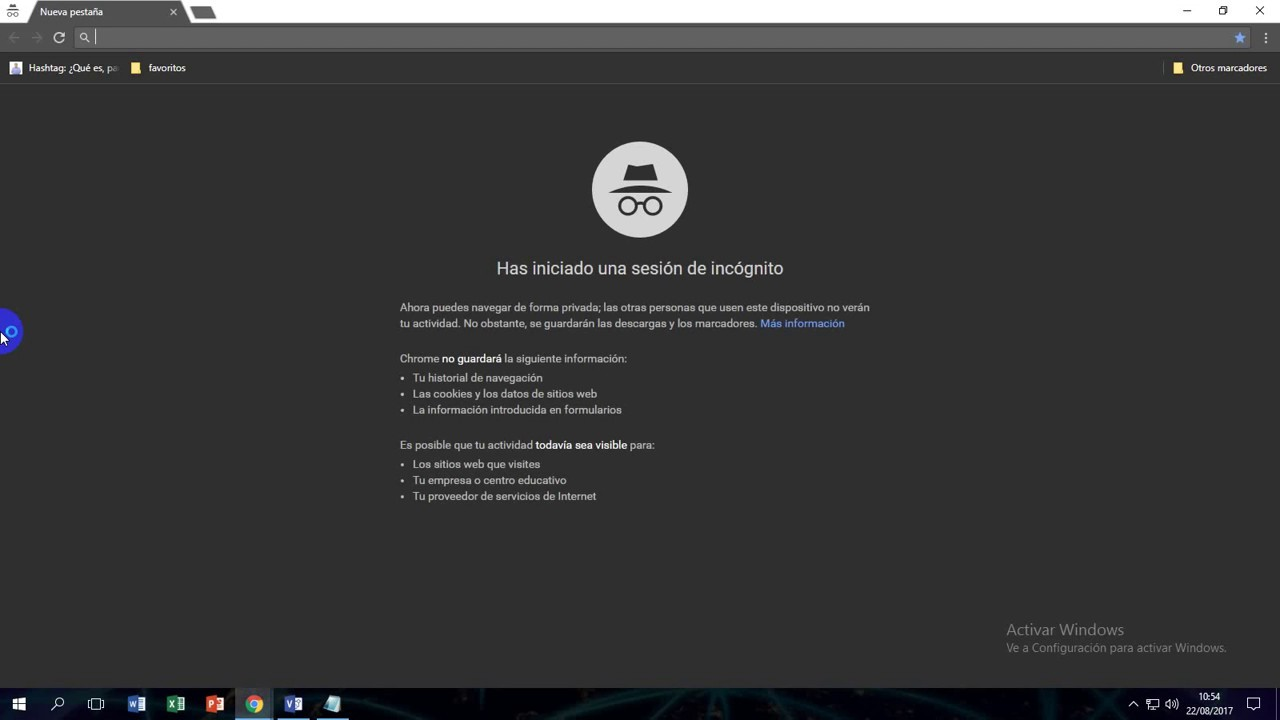
\includegraphics[width=1\linewidth]{images/navegacion-privada} 

}

\caption{Navegación privada navegar Google Chrome.}\label{fig:unnamed-chunk-4}
\end{figure}

Ten en cuenta que no es lo mismo navegar privadamente que navegar de forma anónima por Internet, lo que requiere de otras herramientas como \href{https://www.torproject.org/}{TOR}.

El uso de la navegación privada resulta conveniente en los siguientes supuestos:

\begin{itemize}
\tightlist
\item
  Transacciones económicas.
\item
  Utilización de un ordenador de terceros.
\item
  Resultados ``puros'' del motor de búsquedas.
\end{itemize}

También existen navegadores que protegen tu privacidad sin necesidad de activar la navegación privada, como por ejemplo, \href{https://www.epicbrowser.com/}{Epic}, \href{https://brave.com/es/}{Brave} e incluso buscadores como \href{https://duckduckgo.com/}{DuckDuckGo}.

\hypertarget{vpn-red-privada-virtual}{%
\section{VPN (Red privada virtual)}\label{vpn-red-privada-virtual}}

Otra manera más de proteger tu privacidad, es hacer uso de una VPN (son las siglas de Virtual Private Network) \citep{AVAST-vpn}.

Las VPN, son una tecnología de red que permiten una extensión de tu conexión local o LAN, permitiendo conectar varios dispositivos como si se encontrasen físicamente en el mismo lugar. Entre sus ventajas está la de ofrecer una mayor privacidad al ocultar tu localización, pero también, y este el caso que nos compete, el que parezca que tu conexión esté realizándose en otro país concreto, con lo que uno se puede saltar censuras o acceder a contenidos de servicios locales.

Su principal particularidad es que se trata de una conexión segura y cifrada. Esto hace que no sea posible conocer la información que viaja en la petición que se realiza, así como tampoco la IP pública que identifica nuestro dispositivo, ya que la conexión se realiza a través de los muchos router VPN.

Las VPN suelen ser aplicaciones o extensiones de terceros, aunque el navegador \href{https://www.opera.com/es}{OPERA} lo trae por defecto, lo único que tendrás que hacer es activarla desde sus opciones, y se creará una conexión cifrada entre tu dispositivo y un servidor VPN para esconder tu ubicación real.

\hypertarget{cookies}{%
\section{Cookies}\label{cookies}}

Una cookie es un fichero que guarda nuestro navegador, donde se almacenan pequeñas cantidades de datos, de manera que el sitio web puede consultar la actividad previa del navegador.

Su propósito principal es identificar al usuario almacenando su historial de actividad de un sitio web específico, de manera que se le pueda ofrecer el contenido más apropiado según sus hábitos. Esto quiere decir que cada vez que visitas una página web por primera vez, se guarda una cookie en el navegador con un poco de información. Luego, cuando visitas nuevamente la misma página, el servidor pide la misma cookie para arreglar la configuración del sitio y hacer la visita del usuario tan personalizada como sea posible \citep{cookies-navegador}.

Existe la opción de navegar sin cookies gracias a las sesiones privadas que tienen los distintos navegadores, como has podido ver en el apartado anterior. De esta forma no se almacenará ningún tipo de información en tu ordenador cuando navegues en una web y del mismo modo tampoco recordará nada después al volver a navegar de nuevo.

Es importante que con frecuencia elimines las cookies, ya que como ya sabes manejan información privada y además ocupan espacio en tu dispositivo. Existen dos formas manuales de hacerlo. La primera de ellas es desde el menú de opciones del propio navegador y la otra es con un software específico para tal cometido, como por ejemplo \href{https://www.ccleaner.com/es-es}{Ccleaner}. Pero si quieres automatizar esta tarea, practicamente todos los navegadores disponen de una configuración para que una vez cierres el navegador se realice una limpieza de manera automática. La siguiente imagen te muestra la opción que debes buscar en el navegador Google Chrome, para ello ve al Menu del navegador entra en Configuracíón luego Privacidad y seguridad a continuación Cookies y finalmente Borrar las cookies y los datos de sitios al salir de Chrome, pero debes tener en cuenta que las ubicaciones pueden variar con las actualizaciones. Si usas otro navegador puede ser que varíe la ruta de acceso, pero a grandes rasgos suelen ser muy parecidas y también se acceden a ellas a través del menú de opciones.

\begin{figure}

{\centering 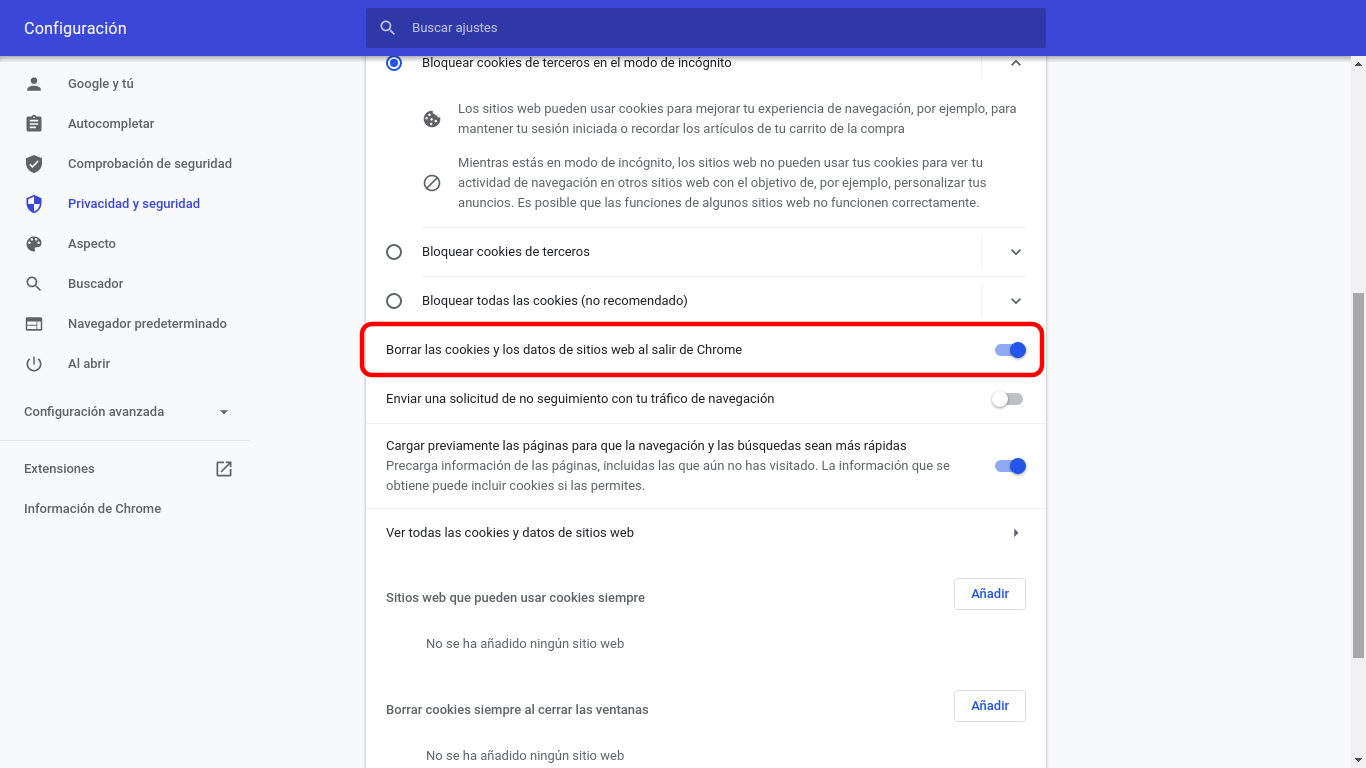
\includegraphics[width=1\linewidth]{images/delete-cookies-when-leave-chrome-browser} 

}

\caption{Eliminar cookies automáticamente al cerrar Google Chrome.}\label{fig:unnamed-chunk-5}
\end{figure}

Por otro lado si quieres deshacerte de la incómoda notificación de cookies de las web, puedes instalar en el navegador el plugin \href{https://www.i-dont-care-about-cookies.eu/}{I don't care about cookies} o este otro \href{https://ninja-cookie.com/}{Ninja cookie}, elige el que más te guste.

Si quieres más información detallada sobre las cookies visita este enlace \href{https://www.osi.es/es/actualidad/blog/2019/09/11/por-que-borrar-las-cookies-del-navegador}{por qué borrar las cookies} y este otro \href{https://www.osi.es/es/actualidad/blog/2018/07/18/entre-cookies-y-privacidad}{tipos de cookies, cofiguración y consejos} de la Oficina de Seguridad del Internauta donde las analizan con más detalle.

\hypertarget{permisos-cuxe1mara-micruxf3fono-y-localizaciuxf3n.}{%
\section{Permisos cámara, micrófono y localización.}\label{permisos-cuxe1mara-micruxf3fono-y-localizaciuxf3n.}}

Una práctica muy saludable en el uso de la cámara o webCam e incluso el micrófono, es tenerla tapada cuando no la estés usando y si no fijate en la foto se muestra a continuación que le tomaron a Mark Zuckerberg.

\begin{figure}

{\centering 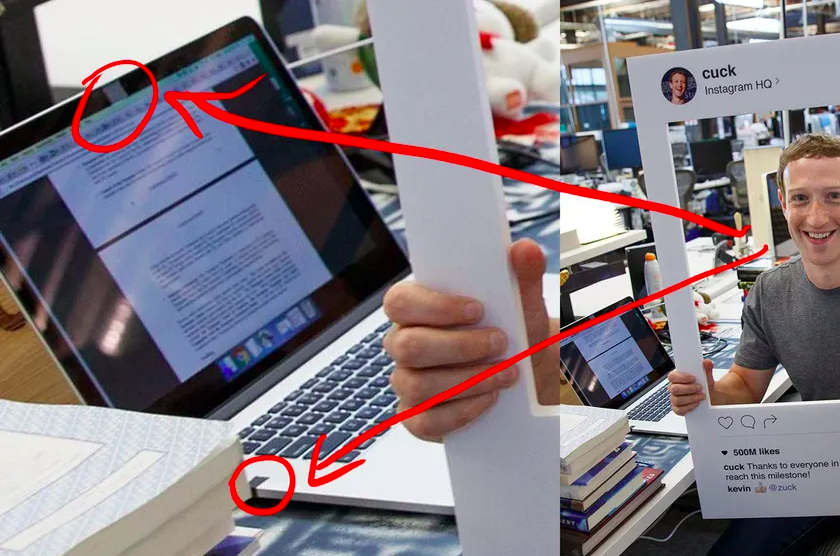
\includegraphics[width=1\linewidth]{images/webca-mark-zuckerberg} 

}

\caption{WebCam y micrófono del ordenador tapados.}\label{fig:unnamed-chunk-6}
\end{figure}

Para tener el control total sobre las funcionalidades de cámara, micrófono y ubicación, debes establecer los permisos en la opción de Preguntar, lo verás más claramente en la imagen que se muestra más abajo. Para establecer estos parámetros existen dos maneras de hacerlo, uno de ellas es a través de la opciones que te da el menú de configuración del propio navegador, y para ello debes ir a Menú navegador, buscar Configuracíón, después Privacidad y seguridad, a continuación Configuración de sitios web y finalmente Permisos y como ya se indicó en el caso de borrado de cookies automático, debes tener en cuenta que las ubicaciones pueden variar con las actualizaciones que reciba el navegador.

\begin{figure}

{\centering 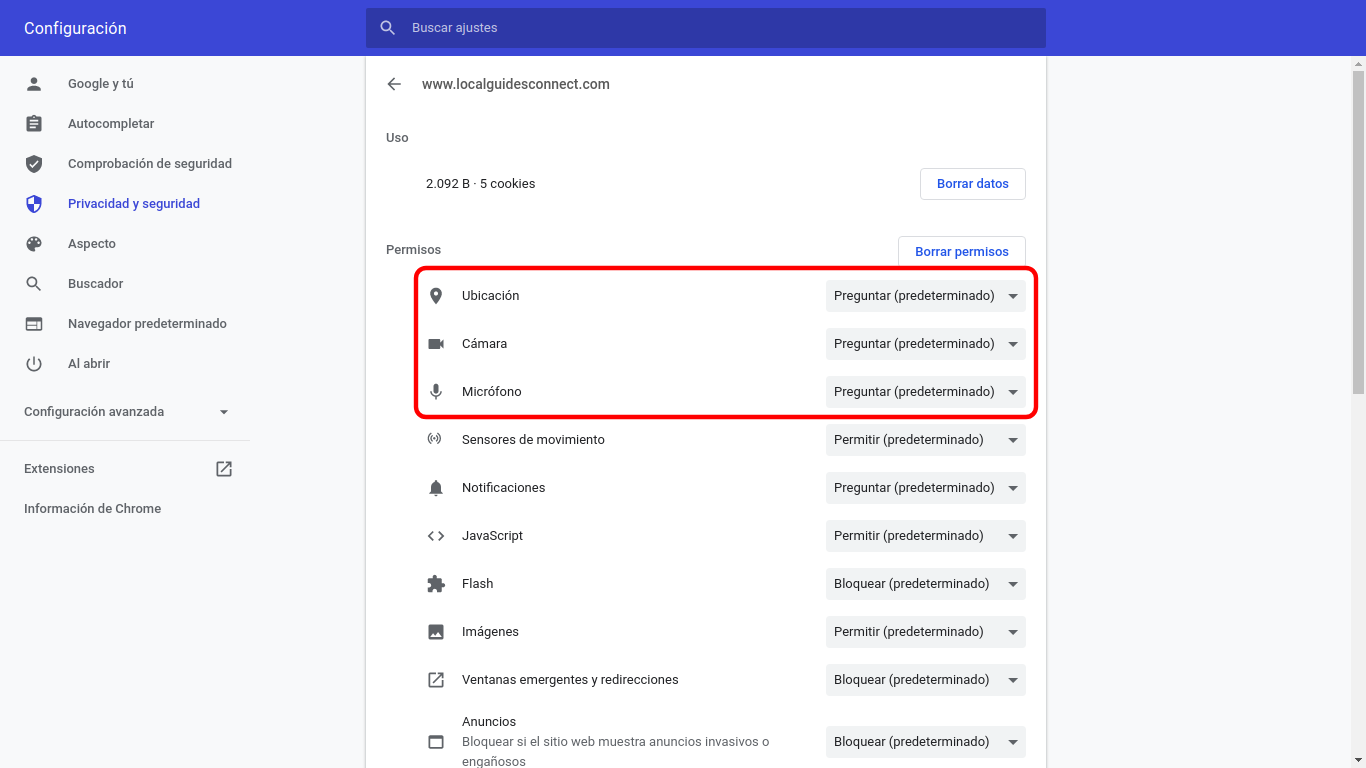
\includegraphics[width=1\linewidth]{images/permition-settings} 

}

\caption{Ajustes permisos cámara, micrófono y ubicación desde el menú de opciones del navegador.}\label{fig:unnamed-chunk-7}
\end{figure}

Aunque estos permisos son los más importantes cuando navegas por internet, si te fijas en la figura 2.4 verás que no son los únicos y que entre éstos se encuentran los de notificaciones o los de ventanas emergentes entre otros.

La otra forma es más sencilla e incluso te permite cambiar los permisos directamente desde el navegador sin tener que ir al menú de opciones y esto lo tienes haciendo click en el candado de la barra de direcciones. Se trata del mismo candado que nos acredita que estamos ante una web segura. Puedes verlo en la siguiente imagen.

\begin{figure}

{\centering 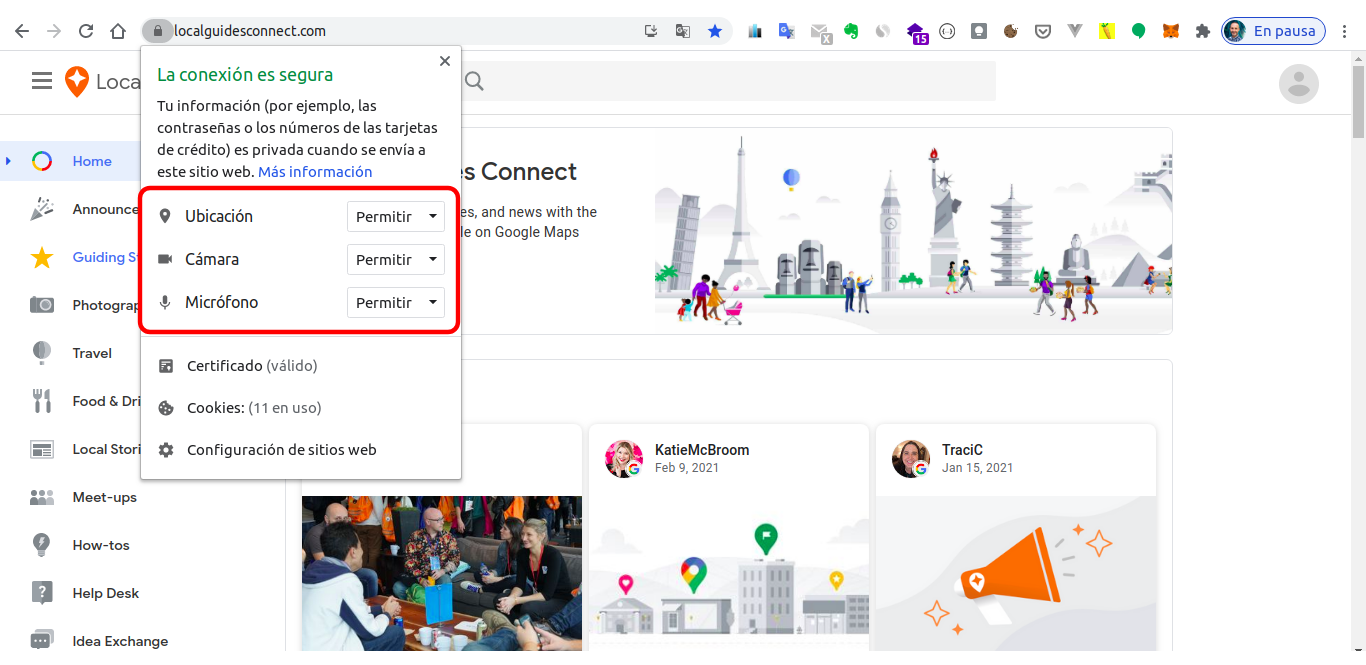
\includegraphics[width=1\linewidth]{images/permitions-setting-from-browser} 

}

\caption{Ajustes permisos cámara, micrófono y ubicación desde el candado de la barra de direcciones.}\label{fig:unnamed-chunk-8}
\end{figure}

Para concluir, no debes olvidar que con las aplicaciones móviles sucede lo mismo, y que puedes gestionarlos de igual manera desde ajustes del dispositivo. Visita los siguientes enlaces dependiendo de tu smartphone, \href{https://support.google.com/android/answer/9431959?hl=es}{cambiar los permisos de las aplicaciones en teléfonos Android} o \href{https://support.apple.com/es-es/guide/iphone/iph251e92810/ios}{controlar el acceso a la información en las apps en el iPhone}. En el siguiente enlace, \href{https://www.osi.es/sites/default/files/docs/c5-eg-permisos-apps-riesgos.pdf}{permisos aplicaciones móviles} encontrarás una tabla con los permisos y los riesgos que entrañan.

\hypertarget{la-nube}{%
\section{La nube}\label{la-nube}}

Como ya sabrás el almacenamiento en la nube, es el almacenamiento de datos en servidores por lo general aportados por terceros y que gracias a esto, puedes disponer de ellos desde cualquier lugar y dispositivo, con solo tener conexión a internet y conectarte al servicio donde están alojados tus datos. De esta manera ya no es necesario llevar contigo el dispositivo físico donde tienes almacenada tu información. Algunos de estos servicios más conocidos son \href{https://www.google.com/intl/en_in/drive/}{Google drive},\href{https://www.microsoft.com/en-us/microsoft-365/onedrive/online-cloud-storage}{One drive} o \href{https://www.dropbox.com/}{Dropbox} entre otros.

Antes de decidirte por cuál de los proveedor de servicio en la nube debes decantarte, ten en cuenta los siguientes:

\begin{itemize}
\item
  Donde va a estar ubicada tu información. Esto te permitirá conocer la legislación y
  garantías de protección de tus datos en el país donde se encuentren.
\item
  Saber si la plataforma comparte información con terceros o no.
\item
  Si la web cuenta con certificado digital y es accesible mediante https.
\item
  Mecanismos de cifrado, ya que éstos maximizan la seguridad de los datos.
\item
  Políticas de privacidad.
\end{itemize}

De otro lado también puedes tomar tus propias medidas de seguridad cifrando tu datos antes de subirlos. Para ello puedes usar esta herramienta llamada \href{https://cryptomator.org/}{cryptomator}.

En este enlace encontrarás un estudio completo de los diferentes \href{https://www.osi.es/sites/default/files/docs/osi_servicios_nube.pdf}{servicios de almacenamiento en la nube} y sus características.

A la hora de compartir tus datos alojados en la nube debes tener en cuenta que solo es recomendable compartirlos con personas de confianza, ya que de lo contrario podrían hacer un mal uso de ello, o simplemente una mala gestión que provoque la pérdida de la información.

\hypertarget{correo-electruxf3nico-y-apps-de-mensajeruxeda}{%
\section{Correo electrónico y apps de mensajería}\label{correo-electruxf3nico-y-apps-de-mensajeruxeda}}

El correo electrónico es uno de los servicios web que más se suele utilizar. Es por ello que debes saber que muchos de lo gestores de emails que son utilizados a diario, no aplican estrictas políticas de privacidad, por lo que tus correos podrías ser leídos y rastreados no solo por terceros con intenciones poco saludables sino también por éstos mismos servicios de correo.

Esto no tiene por que ser un inconveniente si no envías información sensible, pero si no es el caso quizá preferirías usar un gestor de correos que sí te garantice una privacidad completa en tus envíos. De ser este tu caso puedes usar \href{https://protonmail.com/}{Protonmail} o \href{https://tutanota.com/es/}{Tutanota} que si tienen en cuenta este aspecto, aunque no son los únicos. En el siguiente enlace tienes una lista de otras \href{https://blogthinkbig.com/alternativas-gratuitas-gmail-outlook-privacidad}{alternativas de emails privadas}.

Si por el contrario prefieres ser tu quien gestiones esa capa de privacidad adicional, puedes optar por hacer uso de otras herramientas de encriptado que podrás ver en este artículo de \href{https://www.osi.es/es/actualidad/blog/2019/07/31/como-encriptar-y-proteger-tu-correo-electronico}{cómo encriptar y proteger tu correo electrónico}.

Si además quieres saber si tu cuenta de correo ha sido comprometida, puedes saberlo a través de la siguiente plataforma \href{https://haveibeenpwned.com/}{haveibeenpwned}.

Con respecto a las aplicaciones de mensajería instantánea debes tener en cuenta que sucede lo mismo que con los correos electrónicos. A pesar que la mayoría de ellas, incluida la más popular de todas (whatsApp) disponen de capas de privacidad que la hacen confiable, a veces no podemos estar totalmente seguros de no estar sometidos a un seguimiento por parte de éstas. Es por ello que las aplicaciones como \href{https://telegram.org/}{telegram} y \href{https://signal.org/es/}{signal} nacen con el propósito de no inmiscuirse en el uso que haces de la aplicación.

\hypertarget{gestiuxf3n-de-la-seguridad-en-equipos-fuxedsicos}{%
\chapter{Gestión de la seguridad en equipos físicos}\label{gestiuxf3n-de-la-seguridad-en-equipos-fuxedsicos}}

\hypertarget{gestionando-la-seguridad-en-los-equipos}{%
\section{Gestionando la seguridad en los equipos}\label{gestionando-la-seguridad-en-los-equipos}}

Para poder tener la tranquilidad de que tus equipos tales, como el ordenador, la tablet, el smartphone, el router, etc., estén a salvo de ataques o pérdidas de datos, entre otras, debes mantener una seguridad robusta y confiable en tus equipos.

A lo largo de esta unidad veras que debes hacer y las precauciones que debes tomar para que tus equipos e información estén seguros y a salvo de ciberataques.

\hypertarget{equipo-local-y-dispositivos-muxf3viles}{%
\section{Equipo local y dispositivos móviles}\label{equipo-local-y-dispositivos-muxf3viles}}

Una cuenta de usuario es el conjunto de información perteneciente a un usuario concreto. De esta forma indica al sistema operativo los archivos y carpetas a los que dicho usuario tiene acceso así como la posibilidad de realizar cambios y configuraciones personales \citep{OSI-cuentas}.

Las pautas de seguridad que vas a ver a continuación te van a ser útil, tanto para ordenadores como cualquier tipo de dispositivo móvil, smartwatch y demás.

Todos los equipos informáticos funcionan con una cuenta de usuario, única y personal. Luego una vez, hayas creado la tuya, solo tú debes hacer uso y disfrute de ella. En los ordenadores personales existe la posibilidad de crear varias cuentas de usuarios. Una vez éstas están creadas solo son accesibles mediante contraseña y aunque solo sirva para no olvidarlo, nunca debes de compartida.

Desde aquí podrás acceder a cómo \href{https://support.microsoft.com/es-es/windows/crear-una-cuenta-de-administrador-o-de-usuario-local-en-windows-10-20de74e0-ac7f-3502-a866-32915af2a34d}{crear cuenta de usuario en windows} y \href{https://support.apple.com/es-es/guide/mac-help/mtusr001/mac\#:~:text=A\%C3\%B1adir\%20un\%20usuario,en\%20\%E2\%80\%9CUsuarios\%20y\%20grupos\%E2\%80\%9D.\&text=Si\%20el\%20candado\%20situado\%20en,bajo\%20la\%20lista\%20de\%20usuarios}{crear cuenta de usuario en Mac}.

Si tu equipo es compartido con varias personas, puede que te interese crear distintas cuentas de usuarios con distintos niveles de privilegios. Si no las gestionas
adecuadamente, corres el riesgo de:

\begin{itemize}
\item
  Que terceros puedan acceder a tus archivos y eliminar/modificar información personal, como imágenes, música, documentos importantes, etc.
\item
  Modificar configuraciones de seguridad o usabilidad de tu sistema, como, por ejemplo, desactivar el antivirus o firewall.
\item
  Conectarse a determinados servicios con tus credenciales, como el correo electrónico o red social.
\end{itemize}

Además puedes gestionar las \href{https://support.microsoft.com/es-es/windows/las-opciones-de-inicio-de-sesi\%C3\%B3n-de-windows-10-y-la-protecci\%C3\%B3n-de-la-cuenta-7b34d4cf-794f-f6bd-ddcc-e73cdf1a6fbf}{opciones de inicio de sesión en windows} y las \href{https://support.apple.com/es-es/guide/mac-help/mtusr005/mac}{opciones de inicio de sesión en Mac} lo que te permitirá tener un mayor control sobre tu inicio de sesión.

\begin{figure}

{\centering 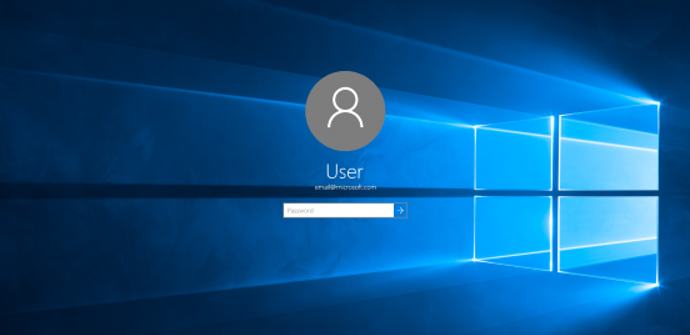
\includegraphics[width=1\linewidth]{images/cuenta-usuario-windows-10} 

}

\caption{Cuenta de usuario windows 10.}\label{fig:unnamed-chunk-9}
\end{figure}

\hypertarget{router}{%
\section{Router}\label{router}}

Un router es un dispositivo que proporciona conectividad a nivel de red. Su función principal consiste en enviar o encaminar paquetes de datos de una red a otra, es decir, interconectar subredes, entendiendo por subred un conjunto de máquinas IP que se pueden comunicar. Además de ser el dispositivo que nos proporciona un punto de acceso Wi-Fi

Dispone de varios niveles de seguridad y estándares de cifrado, para que nadie pueda acceder a nuestra red y poder alcanzar cualquier dispositivo a través d la Wi-Fi.

Ordenados de menor a mayor grado de cifrado:

\begin{itemize}
\tightlist
\item
  \href{https://es.wikipedia.org/wiki/Wired_Equivalent_Privacy}{WEP} (Wired Equivalent Privacy)
\item
  \href{https://es.wikipedia.org/wiki/Wi-Fi_Protected_Access}{WPA} (Wi-Fi Protected Access)
\item
  \href{https://es.wikipedia.org/wiki/WPA2}{WPA2} (Wi-Fi Protected Access 2)
\item
  \href{https://es.wikipedia.org/wiki/WPA3}{WPA3} (Wi-Fi Protected Access 3)
\end{itemize}

Es importante que uses un nivel de seguridad WPA2 como mínimo, con el que vas a poder establecer una contraseña de hasta 63 caracteres en lugar de los máximos 29 de la WEP.

Para establecer una capa más de seguridad puedes realizar un \href{https://es.wikipedia.org/wiki/Filtrado_MAC}{filtrado MAC} (Media Access Control). Un filtra MAC consiste en la creación de una lista de dispositivos que tienen permiso para acceder al router, a pesar de que un tercero haya podido obtener la clave wifi.

Es igualmente importante que cambies la clave que el router trae por defecto. Este enlace te llevará a un \href{https://bandaancha.eu/generador-claves-wifi}{generador de claves Wi-Fi} donde podras crear de forma automática una clave Wi-Fi segura y robusta.

También es una buena práctica cambiar el nombre que la Wi-Fi trae por defecto, esto despistará a aquellos que puedan tener una lista de claves de acceso de las diferentes operadoras que existen en el mercado.

Otro aspecto a tener en cuenta es deshabilitar la opción \href{https://es.wikipedia.org/wiki/Wi-Fi_Protected_Setup}{WPS} (Wifi Protected Setup) en el router. Esta función te permite conectar el ordenador o dispositivo a la Wi-Fi del router sin tener que escribir la contraseña cuando eliges tu red Wi-Fi desde el dispositivo. Se trata de un botón físico que traen algunos router y que al pulsarlo conecta el dispositivo de forma automática. Esta funcionalidad es muy práctica pero conlleva el riesgo de que cuando pulsas este botón estás abriendo la Wi-Fi, lo que significa que inhabilitas todas las medidas de seguridad que tengas configuradas para la conexión. Si decides deshabilitarla puedes hacerlo desde la configuración de tu router y normalmente vas a encontrarlo en los apartados Wireless o Network de la interfaz web \citep{wps}.

Para realizar cualquiera de las configuraciones propuestas en este apartado va a necesitar acceder a la interfaz de tu router y para ello, necesitarás saber la dirección IP de acceso. Esta te será facilitada por tu operador.

Si quieres una buena guía para conocer a fondo los entresijos del router pasate por \href{https://www.osi.es/sites/default/files/docs/guia_router/osi-guia-tu-router-tu-castillo.pdf}{tu router tu castillo}.

\hypertarget{actualizaciones}{%
\section{Actualizaciones}\label{actualizaciones}}

Las actualizaciones de seguridad o parches son elaboradas por los desarrolladores y fabricantes de productos informáticos. Estos pueden tardar desde un día hasta meses para publicar un parche, en función del tipo de vulnerabilidad, dispositivos a los que afecte y otros criterios. Aunque también se realizan para mejoras de otras naturalezas, como, rendimiento, productividad, etc.

Tener actualizados los dispositivos es una medida más de seguridad. Para ello debes actualizarlos cada vez que el dispositivo lo solicita o en su defecto buscar una actualización disponible.

Las actualizaciones no solo corresponden al Hardware (ordenadores, smartphones, etc.), sino que también han de ser realizados en el software (programas), navegadores, antivirus, etc.

La principal función de las actulizaciones son las de mejorar tanto la funcionalidad como la seguridad de los dispositivos o software \citep{OSI-actualizaciones}.

\hypertarget{antivirus-antimalware-antispyware-y-firewall}{%
\section{Antivirus, antimalware, antispyware y firewall}\label{antivirus-antimalware-antispyware-y-firewall}}

Aunque a priori pudiese parecer lo mismo, los antivirus, antimalware, antispyware y firewall, cumple funciones diferentes, pero con un mismo fin, mantener la seguridad de nuestros equipos. La mayoría de estos tipos de software los puedes encontrar en dos modalidades: gratuita y de pago \citep{software-seguridad}.

\begin{itemize}
\item
  Antivirus: Es un programa que detecta la presencia de virus informáticos (software malicioso que altera el funcionamiento normal del ordenador sin que el usuario lo sepa o consienta) y los elimina o repara. Algunos ejemplos de antivirus son: \href{https://www.avira.com/es}{Avira}, \href{https://www.avast.com/es-es/index\#pc}{Avast}, \href{https://www.avg.com/es-es/homepage\#pc}{AVG}, \href{https://www.virustotal.com/gui/}{Virus Total} (online), entre muchos más.
\item
  Firewall o cortafuegos: Es una parte de la red o el sistema que se realiza para bloquear accesos no autorizados y permitiendo los que sí lo están. Se pueden hacer por medio de software o hardware, y permiten una mayor protección a las redes, especialmente importante en empresas que cuentan con datos que han de ser bien protegidos. El \href{https://en.wikipedia.org/wiki/Windows_Firewall}{firewall} más conocido es el Windows.
\item
  Antispyware: Es un conjunto de herramientas que sirven para prevenir y eliminar Spywares (espías o programas que recopilan información del ordenador para transmitirla a otras personas sin el consentimiento ni conocimiento del propietario del ordenador). Algunos ejemplos de antispyware son: \href{https://www.safer-networking.org/}{SpyBot}, \href{https://www.superantispyware.com/}{SuperAntiSpyware}, \href{https://www.brightfort.com/spywareblaster.html}{SpywareBlaster}.
\item
  Antimalware: Es un software encargado de eliminar el software malicioso (malicious-software, malware) del ordenador tras un minucioso análisis del sistema. Algunos ejemplos de antimalware son: \href{https://www.infospyware.com/antimalware/hijackthis/}{HiJackThis}, \href{https://www.malwarebytes.com/}{Anti-malware}.
\end{itemize}

Dependiendo de las necesidades pueden ser usados uno o varios, ya que son complementarios entre sí.

Antes de decidir que herramientas de las anteriormente expuestas va a usar, puedes hacer una búsqueda e informarte sobre las opciones disponibles, ya que existen soluciones de todo tipo y para todos los gustos, gratuitas, de pago, para ordenadores, para smartphones. Desde la \href{https://www.osi.es}{Oficina de Seguridad del Internauta} ponen a tu disposición este \href{https://www.osi.es/es/herramientas-gratuitas?herramienta_selec\%5B0\%5D=115}{listado de Antivirus gratuitos}, para que puedas elegir el que mejor se adapte a tus necesidades. Pero no olvides nunca de asegurarte muy bien que estás ante un producto legítimo y descargarlo siempre de la web oficial.

\hypertarget{copias-de-seguridad}{%
\section{Copias de seguridad}\label{copias-de-seguridad}}

Una copia de seguridad o backup en informática es una copia de los datos originales que se realiza con el fin de disponer de un medio para recuperarlos en caso de su pérdida. Las copias de seguridad son útiles ante distintos eventos y usos: recuperar los sistemas informáticos y los datos de una catástrofe informática, natural o ataque; restaurar una pequeña cantidad de archivos que pueden haberse eliminado accidentalmente, corrompido, infectado por un virus informático u otras causas \citep{WIKI-copias-seguridad}.

Simplificando el sistema de copias de seguridad que en algunas ocasiones puede llegar a ser complejo, están los siguiente:

\begin{itemize}
\item
  Completas: Del sistema operativo completo, de esta forma al restaurar la copia, dispondremos de nuevo de toda la configuración a nivel de S.O., software instalado, carpetas y archivos. Para este cometido vamos a necesitar de programas de terceros, algunos de ellos con versiones gratuitas y de pago, ejemplo de estos son: \href{https://www.acronis.com/}{Acronis}, \href{https://www.aomeitech.com/}{AOMEI}, \href{https://www.easeus.com/}{EaseUS}. Aunque más abajo verás que también pueden hacerse nativamente.
\item
  Parciales: En este escenario lo que se hace es salvaguardar las carpetas y archivos personales. Como por ejemplo, carpetas con fotografías, documentos personales y demás.
\end{itemize}

Y las copias pueden ser mantenidas:

\begin{itemize}
\item
  En almacenamientos externos: Tales como disco duros externos, DVD, entre otros. De esta forma podemos custodiarlos a buen recaudo.
\item
  En la nube: Estos son servicios de terceros accesibles online, ejemplo de ello son: \href{https://www.backblaze.com/home-1.html}{BackBlaze}, \href{https://www.carbonite.com/}{Carbonite}, siendo estos especializados en backups. Pero si tus copias de seguridad se limitan a tus carpetas y archivos personales puedes usar un servicio en la nube, como \href{https://www.google.com/intl/en_in/drive/}{Google Drive}, \href{https://www.microsoft.com/en-us/microsoft-365/onedrive/online-cloud-storage}{Onedrive} o \href{https://www.dropbox.com/}{Dropbox}.
\end{itemize}

Las copias de seguridad debes realizarlas con la frecuencia que sea necesaria para garantizar tu nivel de seguridad \citep{tipos-copia-seguridad}.

Puedes crear una copia de seguridad de tu sistema fácilmente ya que tanto Windows como Mac traen esta opción de forma nativa, solo necesitaras disponer de un dispositivo externo de almacenamiento en el que puedas guardar la copia con espacio de almacenamiento suficiente.

Para Windows tienes a información en \href{https://support.microsoft.com/es-es/windows/realizar-y-restaurar-una-copia-de-seguridad-del-pc-ac359b36-7015-4694-de9a-c5eac1ce9d9c}{realizar y restaurar una copia de seguridad del PC}. Y en dispositivos Apple existe la opción de \href{https://support.apple.com/es-es/mac-backup}{cómo hacer copias de seguridad en Mac}.

Una práctica muy recomendable a la hora de hacer copias de seguridad es seguir la estrategia 3-2-1 \citep{INCI-copia-3-2-1} y que consiste en:

\begin{itemize}
\item
  Mantener 3 copias de seguridad: una principal con la que trabajar y dos de backups.
\item
  Mantener la información en 2 tipos de almacenamiento distintos, por ejemplo, en un disco duro y en la nube.
\item
  Mantener 1 copia de seguridad fuera de nuestra casa.
\end{itemize}

Las copias de seguridad no son solo exclusivas de los PCs o portátiles, sino que también debes contemplarlas en tus dispositivos móviles. Android pone a tu dispoción el recurso de cómo \href{https://support.google.com/android/answer/2819582?hl=es\&visit_id=637514255756661953-3969236140\&rd=1}{crear copias de seguridad o restaurar datos de un dispositivo Android} y Apple el de \href{https://support.apple.com/es-es/HT203977}{cómo hacer una copia de seguridad del iPhone, iPad y iPod touch}.

\hypertarget{cifrado-o-encriptado-de-unidades-de-almacenamiento}{%
\section{Cifrado o encriptado de unidades de almacenamiento}\label{cifrado-o-encriptado-de-unidades-de-almacenamiento}}

Cifrar o encriptar tus discos duros ya sean externos o internos del ordenador o el encriptado de un simple Pendrive o USB es cada día más necesario para protegernos contra los amigos de lo ajeno, ya que aunque te sustrayecen el ordenador o cualquier otro dispositivo, no podrían acceder a la información puesto que se encuentra bajo esta capa de seguridad robusta que es la encriptación.

El cifrado de dispositivos es una tecnología que cifra todos los datos almacenado en discos duros o cualquier otro dispositivo de almacenamiento externo, con sofisticadas funciones matemáticas recogidas en lo que se conoce como \href{https://es.wikipedia.org/wiki/Criptografía}{criptografía}. De manera que para poder acceder a la información almacenada en el disco duro o pendrive en necesario tener la contraseña o clave de acceso \citep{cifrado}.

Exiten varias herramientas en el mercado para este cometido como las detalladas a continuación:

\begin{itemize}
\item
  \href{https://docs.microsoft.com/es-es/windows/security/information-protection/bitlocker/bitlocker-overview}{BitLocker}. Software nativo del sistema operativo Windows.
\item
  \href{https://support.apple.com/es-es/HT204837}{FileVault}. Software nativo del sistema opera de macOS.
\item
  \href{https://www.veracrypt.fr}{Veracrypt}.
\item
  \href{https://diskcryptor.org/}{Diskcryptor}.
\item
  \href{https://www.comodo.com/home/internet-security/disk-encryption.php}{Comodo Disk Encryption}.
\end{itemize}

También tienes a tu dispoción el siguiente enlace que te llevará a la revista digital \href{https://computerhoy.com/tutoriales/tecnologia/como-cifrar-disco-duro-memoria-externa-nadie-pueda-acceder-ella-386434}{Computerhoy} donde te explican como encriptar tu ordenador windows o mac.

\hypertarget{gestiuxf3n-de-la-seguridad-en-la-red}{%
\chapter{Gestión de la seguridad en la red}\label{gestiuxf3n-de-la-seguridad-en-la-red}}

\hypertarget{gestionando-la-seguridad-en-la-red}{%
\section{Gestionando la seguridad en la red}\label{gestionando-la-seguridad-en-la-red}}

Como ya viste en la unidad de privacidad y seguridad, la seguridad en internet son todas aquellas precauciones que deben ser tomadas para proteger todos los dispositivos informáticos, así como la red de internet que pueden ser afectados por delincuentes cibernéticos.

Más adelante verás de qué situaciones y amenazas te estás protegiendo si sigues todas estas recomendaciones.

\hypertarget{contraseuxf1as}{%
\section{Contraseñas}\label{contraseuxf1as}}

Una contraseña, clave o password es una forma de autentificación que utiliza información secreta para controlar el acceso hacia algún recurso. La contraseña debe mantenerse en secreto ante aquellos a quien no se le permite el acceso \citep{WIKI-password}.

Y su utilidad consiste en que a aquellos que desean acceder a la información se les solicita una clave o contraseña, si conocen dicha contraseña se les concede el acceso y si no la conocen, se les niega el acceso a la información.

Estas deben ser lo más seguras posibles, para ello deben crearlas bajo las siguientes:

\begin{itemize}
\item
  Debes incluir números.
\item
  Utiliza una combinación de letras mayúsculas y minúsculas.
\item
  Incluye caracteres especiales. Ejemplos: * ? ! @ \# \$ / () \{\} = . , ; :
\item
  Una longitud mayor o igual a 8 caracteres.
\item
  No debes incluir espacios en blanco.
\end{itemize}

Una modalidad de crear contraseñas robustas y fáciles de recordar es la siguiente \citep{OSI-contraseñas}:

\begin{enumerate}
\def\labelenumi{\arabic{enumi}.}
\item
  Elige una extensión de más de 8 caracteres. Ejemplo : Mi cuenta segura
\item
  Pon la primera mayúscula y elimina los espacios en blanco. Ejemplo: MicuentaSegura
\item
  Cambia las letras por números. Ejemplo: M1Cu3nt4S3gur4
\item
  Añade caracteres especiales. Ejemplo: M1Cu3nt4S3gur4!
\item
  Personaliza la clave para cada servicio. Toma las dos primeras letras del servicio, para el caso de Facebook son la F y la A y colocalas una delante y otra detrás. Ejemplo: FM1Cu3nt4S3gur4!A
\end{enumerate}

En la \href{https://www.osi.es/es}{Oficina de Seguridad del Internauta} tienes toda una suit de recursos para crearte la mejor de las contraseñas posible. Accede desde este enlace \href{https://www.osi.es/es/campanas/contrasenas-seguras}{Contraseñas seguras}.

También es recomendable que la cambies cada cierto tiempo, al menos aquellas que sean de mayor importancia.

A su vez también han de ser fáciles de recordar, pero debes de huir de patrones poco seguros y fáciles de adivinar. A continuación, algunos ejemplos de contraseñas que nunca debes utilizar:

\begin{itemize}
\item
  Qwerty
\item
  1234
\item
  Asdfg
\item
  Password
\item
  11111
\item
  Usar datos personales como la fecha de nacimiento, nombre mascota, etc.
\end{itemize}

En el siguiente enlace encontrás una lista de las \href{https://nordpass.com/most-common-passwords-list/}{contraseñas más comunes} que jamás deberías utilizar. Echale un vistazo por si alguna de esas se parece a la tuya.

Algunas reglas y ejemplos para que las contraseñas sean fáciles de recordar los encontrás en estos enlaces:

\begin{itemize}
\item
  \href{https://www.pandasecurity.com/es/mediacenter/seguridad/10-trucos-para-crear-contrasenas-seguras/}{Trucos para crear contraseñas seguras}
\item
  \href{https://www.genbeta.com/seguridad/especial-contrasenas-seguras-consejos-para-mejorar-la-seguridad-de-tus-contrasenas}{Consejos para crear contraseñas seguras}
\end{itemize}

Otras recomendaciones que debes a tener siempre presente son:

\begin{itemize}
\item
  No las compartas con nadie.
\item
  No uses la misma contraseña en diferentes servicios.
\item
  No las almacenes en el navegador.
\item
  Evita usarlas en dispositivos públicos.
\item
  Usa la \href{https://www.osi.es/es/actualidad/blog/2019/02/27/el-factor-de-autenticacion-doble-y-multiple}{verificación en dos pasos} también conocida como autenticación doble.
\item
  Usar \href{https://cloud.google.com/titan-security-key/?hl=es}{security keys}.
\item
  Gestores de contraseñas:

  \begin{itemize}
  \tightlist
  \item
    \href{https://bitwarden.com/}{Bitwarden}
  \item
    \href{https://www.lastpass.com/es/}{LastPass}
  \item
    \href{https://passwords.google.com/}{Google passwords}
  \item
    \href{https://nordpass.com/homepage/}{NordPass}
  \item
    \href{https://www.dropbox.com/es_ES/features/security/passwords}{Dropbox passwords}
  \end{itemize}
\end{itemize}

Para acabar con este apartado puedes comprobar la seguridad y robustez de tu contraseña, con los siguientes recursos online:

\begin{itemize}
\item
  \href{https://www.security.org/how-secure-is-my-password/}{How Secure Is My Password}
\item
  \href{https://password.kaspersky.com/}{Password Check}
\end{itemize}

Por otro lado si eres de las personas que te gusta tener todo bajo control puedes usar este servicio de Google llamado \href{https://www.blog.google/technology/safety-security/google-password-checkup-cross-account-protection/}{Password Checkout} o este otro llamado \href{https://haveibeenpwned.com/Passwords}{Haveibeenpwned Passwords} para averiguar si alguna de tus contraseñas ha sido comprometida.

\hypertarget{protocolo-https}{%
\section{Protocolo https}\label{protocolo-https}}

El Protocolo seguro de transferencia de hipertexto (en inglés: Hypertext Transfer Protocol Secure o HTTPS), es un protocolo de aplicación basado en el protocolo HTTP, destinado a la transferencia segura de datos de Hipertexto, es decir, es la versión segura de HTTP \citep{WIKI-https}.

El sistema HTTPS utiliza un cifrado basado en la seguridad de textos SSL/TLS para crear un canal cifrado.

De este modo se consigue que la información sensible (usuario y claves de paso normalmente) no pueda ser usada por un atacante que haya conseguido interceptar la transferencia de datos de la conexión, ya que lo único que obtendrá será un flujo de datos cifrados que le resultará imposible de descifrar.

Identificar si el protocolo https está activado en el navegador es muy sencillo. Sólo debes fijarte en la parte superior izquierda de tu navegador. Si tu URL inicia con https: //, o bien, antes de la dirección se muestra un candado, estarás navegando con seguridad bajo el protocolo https.

\begin{figure}

{\centering 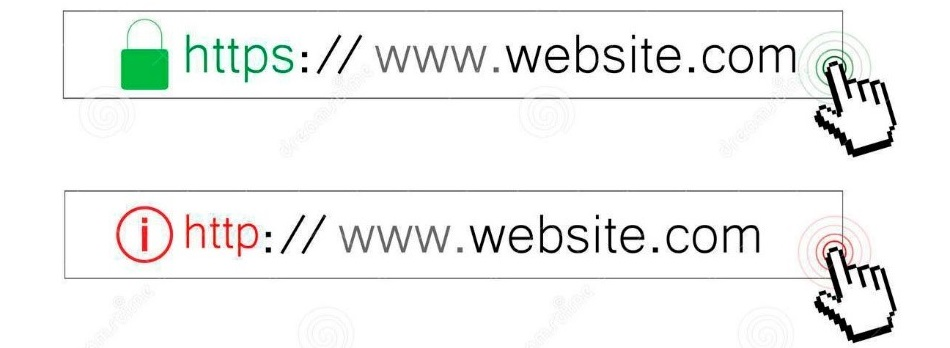
\includegraphics[width=0.75\linewidth]{images/protocolo-https-http} 

}

\caption{Protocolo https vs http.}\label{fig:unnamed-chunk-10}
\end{figure}

Si haces click en el candado, éste te mostrará que se trata de conexión es segura, así como el certificado, cookies y configuración de sitios.

IMPORTANTE: Tener el candado no garantiza que la web sea legítima. Ya que los certificados de cifrado seguro los emiten terceros y los ciberestafadores pueden hacerse igualmente con uno.

\hypertarget{compras-y-transacciones}{%
\section{Compras y transacciones}\label{compras-y-transacciones}}

Para comprar por Internet debes tomar cuantas más precauciones mejor para evitar cualquier tipo de fraude. Los factores a tener en cuenta son los siguientes:

\begin{itemize}
\item
  Evita sitios webs que no te inspiren confianza: Por ello solo debes compras a través de webs y aplicaciones oficiales. Además de buscar valoraciones y opiniones, utilizar plataformas que valoran la reputación online de un portal, como \href{https://www.scamadviser.com/}{Scamadviser}.
\item
  Usa solo plataformas con protocolo HTTPS: Visto en el apartado anterior.
\item
  Utiliza navegación privada: Así evitarás que se registre el historial de navegación.
\item
  Trata de usar pasarelas de pago: Evita en lo posible el uso de tarjetas de crédito y opta por una pasarela de pago, como puede ser \href{https://www.paypal.com/es/home}{PayPal}, te estarás garantizando la compra, además de disponer de protocolos de devolución del importe muy efectivos.
\item
  Haz comprobaciones adicionales:

  \begin{itemize}
  \item
    Comprueba que la web está adherida a alguna plataforma de confianza online, como, por ejemplo, \href{https://www.confianzaonline.es/}{Confianza Online}. Se trata del único sello de calidad que cuenta con los reconocimientos de la Comisión Europea, el Instituto Nacional de Consumo o la Agencia Española de Protección de datos, además de estar respaldado por el Ministerio de Industria, Energía y Turismo. Y acredita que se cumple con los estándares de privacidad y protección de datos de los usuarios entre otros. También existe el \href{https://www.aenor.com/certificacion/tecnologias-de-la-informacion/buenas-practicas-comercio-electronico}{Certificado de comercio electrónico} expedido por Aenor.
  \item
    Verifica que reciben nálisis de seguridad periódicos realizados por plataformas como \href{https://www.mcafeesecure.com/certification}{McAfee Secure}.
  \item
    Asegúrate que disponen de certificados de autenticidad de la web y seguridad de las transacciones como los que ofrece \href{https://es.norton.com/internet-security}{Norton secured} o \href{https://www.comodo.com/home/internet-security/secure-shopping.php}{Comodo secure}.
  \item
    Estos sellos y certificados los encontrarás normalmente en la parte inferior de la web en forma de logos y debes hacer click en ellos para obtener más información sobre la entidad que los expide y la vigencia de éstos, ya que muchas web fraudulentas utilizan sellos falsos.
  \end{itemize}
\end{itemize}

\begin{figure}

{\centering 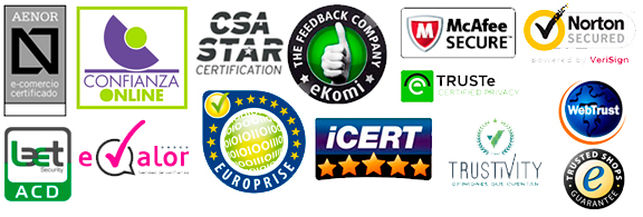
\includegraphics[width=0.75\linewidth]{images/sellos-de-confianza-online} 

}

\caption{Sellos y certificados de comercio online.}\label{fig:unnamed-chunk-11}
\end{figure}

\hypertarget{wi-fi}{%
\section{Wi-Fi}\label{wi-fi}}

Con respecto a la Wi-Fi nos encontramos ante dos escenarios: Wi-Fi propia y Wi-Fi ajena.

Uno de los peligros a los que más expuestos estas con tus equipos portátiles ya sean ordenadores, smartphones, etc., es el de buscar puntos Wi-Fi ajenos. Ya que por lo general suelen ser puntos de accesos a la red gratuitos. En este escenario, existe el riesgo que aun tratándose de una red confiable puede haber sido hackeada por un tercero o que en primera instancia no provenga ni si quiera de una red de confianza. En cualquiera de los dos supuestos, tus dispositivos quedan expuestos y con ello, toda tu información sensible, a merced de ser espiado, robado o extorsionado.

Es por ello que debes tener la precaución de no hacer transacciones de ningún tipo, ni enviar datos sensibles. Es decir, usarla solo en caso de no te quede otra opción o en caso de tener que hacer cualquier búsqueda de carácter trivial.

Es de suponer que si estas en casa con Wi-Fi propia, estas recomendaciones no son tan necesarias. Pero si que sería muy recomendable por tu parte, que tuvieses muy en cuenta las recomendaciones que tienes a tu disposición en el apartado de Router en este manual. Además es conveniente que si no has establecido las capas de seguridad que se recomiendan en ese apartado, hagas una revisión de tu conexión Wi-Fi, por si tienes algún intruso y de ser así poder eliminarlo. Para ello tienes a tu disposición en el \href{https://www.osi.es/es/actualidad/blog}{blog de la Oficina de Seguridad de Internauta} un recurso llamado \href{https://www.osi.es/es/actualidad/blog/2019/09/25/descubre-y-elimina-los-intrusos-de-tu-red-wifi}{descubre y elimina a los intrusos de tu red wifi}.

Lo más recomendable es que siempre que puedas navegues con cable en lugar de Wi-Fi.

\hypertarget{plugins-o-extensiones}{%
\section{Plugins o extensiones}\label{plugins-o-extensiones}}

En informática, un complemento o plug-in es una aplicación (o programa informático) que se relaciona con otra para agregarle una función nueva y generalmente muy específica. Esta aplicación adicional es ejecutada por la aplicación principal e interactúan por medio de la interfaz de programación de aplicaciones. Complemento y plug-in se diferencian en que los complementos son desarrollados por empresas reconocidas y tienen certificado de seguridad y los plug-in pueden ser desarrollados por cualquiera \citep{WIKI-plugin}.

Existen una infinidad de plug-in de diferente naturaleza y para multitud de propósitos. En esta ocasión nos vamos a centrar en los usados por los navegadores, un ejemplo de estos es el archiconocido \href{https://getadblock.com/}{adBlock}, cuya función es la eliminar esos molestos anuncios de algunos portales webs.

Estos pueden estar desarrollados por terceros con intenciones de controlar la información que manejamos en nuestro dispositivo. De ahí que deban proceder de fuentes fiables y que estén configurados para actualizaciones automáticas.

Cada navegador dispone de repositorio de plug-ins o extensiones, que pueden ser consultados y desde donde los puedes instalar y comprobar su fiabilidad, así como consultar las valoraciones.

\begin{figure}

{\centering 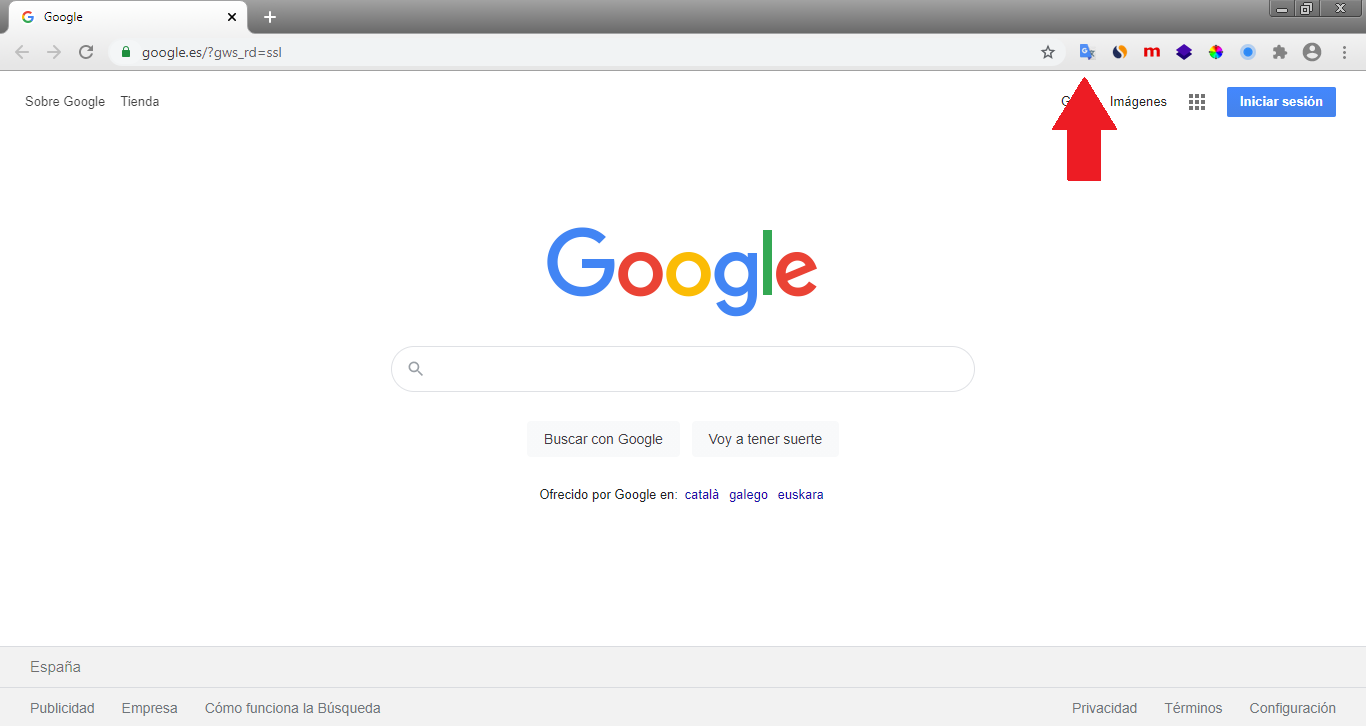
\includegraphics[width=1\linewidth]{images/plugin-navegador} 

}

\caption{Plugin traductor de Google seguido de otros plugin con diferentes funcionalidades.}\label{fig:unnamed-chunk-12}
\end{figure}

Si quieres ampliar tu conocimiento y saber más de plugins y extensiones pasate por el \href{https://www.osi.es/es/actualidad/blog}{blog de la Oficina de Seguridad de Internauta} y lee esta entrada sobre \href{https://www.osi.es/es/actualidad/blog/2019/11/20/extensiones-superpoderes-para-los-navegadores}{extensiones: Superpoderes para los navegadores}.

\hypertarget{descargas}{%
\section{Descargas}\label{descargas}}

Debes de tener muy en cuenta que las aplicaciones o programas deben ser descargadas desde sus sitios oficiales, y no desde otros. Es importante tener siempre presente que, incluso en ocasiones ni si quiera los antivirus reconocen algunas aplicaciones o programas que pudieran contener alguna vulnerabilidad, algún virus o gusano que afecte tu ordenador.

Existen también multitud de webs que en apariencia, ofrecen programas muy mediáticos o de mucha popularidad y que pueden haber sido previamente infectados con algún tipo de código malicioso mediante la modificación o alteración del mismo. Por ello, lo más aconsejable es que descarges las aplicaciones desde las webs oficiales \citep{software-alterado}.

Dentro de todos los tipos de archivos que pueden contener malware, uno de los más comunes es el .EXE. Incluso a la hora de descargar archivos de este tipo nuestro antivirus puede saltar aunque no se trate de una amenaza. Cuando queremos mandar un EXE por e-mail tampoco nos dejan. Es todo un clásico, ya que se trata de un archivo ejecutable que podría instalar software malicioso en nuestro sistema. Hay que tener mucho ojo siempre que gestionemos un archivo de este tipo \citep{exe}.

Es una buena práctica huir de portales de terceros, ya con los instaladores muchso de ellos descargan malware y molestas toolbars.

\hypertarget{cierre-de-sesiones}{%
\section{Cierre de sesiones}\label{cierre-de-sesiones}}

Cuando hagas uso de algún servicio en internet, como por ejemplo, Facebook, Gmail o cualquier otro, lo primero que tienes que hacer es iniciar sesión con tus credenciales.

Si estas en tu dispositivo no pasaría nada si una vez abierta la sesión no la cierras después de haber usado el servicio, pero si por el contrario estas usando un dispositivo ajeno, el servicio quedaría abierto y tus datos expuestos.

Por la razón antes expuesta, es importante que no dejes ninguna sesión abierta.

\hypertarget{sv-two-step-verification-o-verificaciuxf3n-en-dos-pasos}{%
\section{2SV (Two Step Verification) o Verificación en Dos Pasos}\label{sv-two-step-verification-o-verificaciuxf3n-en-dos-pasos}}

La mayoría de cuentas a día de hoy están configuradas para soportar lo que se conoce como SFA (Single Factor Authetication) o Factor de autenticación Simple. Se trata del acceso a cuentas o servicios con el solo uso del usuario y una contraseña, algo que todo el mundo viene haciendo desde hace tiempo. Esto se ha vuelto en gran medida un gran riesgo, ya que si un tercero consigue hacerse con tu contraseña no tendrá ninguna dificultad para tomar el control.

Es por este motivo que cada vez más servicios están implementando lo que se conoce como 2SV (Two Step Verification) o Verificación en Dos Pasos. Este sistema consiste en un código adicional, que suele ser enviado por correo electrónico, SMS, llamada telefónica o App de verificación en dos pasos, justo después de iniciar sesión con tu usuario y contraseña y el cual debe ser ingresado dentro de un determinado lapso de tiempo, (ya que el código expira en poco tiempo), para poder acceder al servicio.

Como puedes ver, los dos pasos son:

\begin{enumerate}
\def\labelenumi{\arabic{enumi}.}
\tightlist
\item
  Usuario y contraseña: Que solo tú conoces.
\item
  Código adicional: Enviado por correo electrónico, SMS, llamada telefónica o App de verificación en dos pasos.
\end{enumerate}

\begin{figure}

{\centering 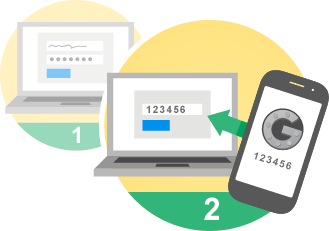
\includegraphics[width=0.4\linewidth]{images/two-step-verification} 

}

\caption{Verificación en dos pasos.}\label{fig:unnamed-chunk-13}
\end{figure}

De esta manera para que los ciberdelicuentes puedan acceder a tu servicio necesitarán la contraseña y el código adicional.

Algunos servicios como la \href{https://www.google.com/landing/2step/?hl=es}{verificación en dos pasos de google} viene de manera nativa y tan solo tienes que activarla. Otros son gestionados a través de correo electrónico, SMS o llamadas telefónicas, como es el caso de algunas entidades bancarias. Y en otros supuestos, aunque la plataforma disponga de dicho servicio necesitarás una aplicación externa como \href{https://support.google.com/accounts/answer/1066447?co=GENIE.Platform\%3DAndroid\&hl=es-419}{Google Autenticator} o \href{https://www.microsoft.com/es-es/account/authenticator}{Microsoft autenticator} entre otras y que se trata de una App de verificación en dos pasos, que te genera el código adicional.

Es extremadamente recomendable que uses este sistema de verificación en la medida que puedas. Recuerda que de un modo u otro la mayoría de servicios y plataformas disponen de esta capa de seguridad. Normalmente las encontrarás en Ajustes y Seguridad. Si quieres más información, en este enlace sobre \href{https://www.osi.es/es/actualidad/blog/2017/01/17/verificacion-en-dos-pasos-que-es-y-como-me-puede-ayudar}{verificación en dos pasos} encontrarás más detalles, además de enlaces hacia las distintas plataformas y redes sociales más populares para que puedas implementarlo.

\hypertarget{mfa-multi-factor-authentication-o-autenticaciuxf3n-de-factores-muxfaltiples}{%
\section{MFA (Multi-Factor Authentication) o Autenticación de Factores Múltiples}\label{mfa-multi-factor-authentication-o-autenticaciuxf3n-de-factores-muxfaltiples}}

La autenticación de factores múltiples \ldots{}

\hypertarget{cifrado-o-encriptaciuxf3n-de-datos}{%
\section{Cifrado o encriptación de datos}\label{cifrado-o-encriptaciuxf3n-de-datos}}

Encriptación de datos \ldots{}

\hypertarget{antibotnet}{%
\section{AntiBotnet}\label{antibotnet}}

Los antibotnet son\ldots{}

\hypertarget{bluetooth-y-nfc}{%
\section{Bluetooth y NFC}\label{bluetooth-y-nfc}}

El bluetooth \ldots{}

\hypertarget{amenazas}{%
\chapter{Amenazas}\label{amenazas}}

\hypertarget{principales-amenazas}{%
\section{Principales amenazas}\label{principales-amenazas}}

En lo referente a la seguridad de nuestros dispositivos debes tener en cuenta la diversidad de amenazas que existen, tales como virus, spywares, troyanos, gusanos y que pueden comprometer tus dispositivos y toda la información que en ellos contengas.

La mayoría de éstos están catalogado como Malware. Un Malware es un tipo de software malicioso con un primer objetivo inicial de infiltrarse en un equipo o sistema informático sin el consentimiento del usuario, para posteriormente actuar sobre él \citep{WIKI-malware}.

En este punto es importante que sepas cuáles son todas y cada una de las amenazas a las que estas expuesto, si no tienes las herramientas y no adoptas una actitud prudente en el uso de los dispositivos y la red.

En unidades anteriores viste que precauciones y herramientas debes adoptar para no correr riesgos. En esta unidad verás cuáles son estas amenazas y como llegan a tus dispositivos.

Las amenazas vienen de la mano de perfiles a los que conoces como hacker, ciberdelicuente, pirata informático, etc. Pero cabe destacar que estos conceptos no son lo mismo. Por lo tanto:

\begin{itemize}
\item
  Hacker: Es un perfil técnico especializado en seguridad informática, y cuyo propósito es investigar y solucionar fallos de seguridad a los fabricantes de dispositivos y software.
\item
  Ciberdelincuente o pirata informático: Es también un perfil técnico como el anterior, pero que en este caso aprovecha las vulnerabilidades de los dispositivos para su propio beneficio a través de actividades delictivas. Su principal actividad suele ser el fraude electrónico utilizando técnicas de phishing o spam.
\end{itemize}

\hypertarget{virus}{%
\section{Virus}\label{virus}}

Un virus es un programa informático diseñado para infectar archivos u ocasionar efectos molestos, destructivos e incluso irreparables en tu ordenador, dañando hardware, software y archivos \citep{PANDA-virus}.

Los virus tienen diferentes vías de entrada a tus equipos, como por ejemplo:

\begin{itemize}
\item
  Utilización de una memoria USB previamente infectada.
\item
  Descarga de contenidos mediante redes de compartición P2P, u otras fuentes poco fiables.
\item
  Apertura de algún fichero adjunto en un correo electrónico.
\item
  Al visitar a una web maliciosa y pulsar sobre alguna dirección acortada que se publican en redes sociales y que en realidad no sabes a qué páginas web te puede llevar.
\end{itemize}

\hypertarget{gusanos-informuxe1ticos}{%
\section{Gusanos informáticos}\label{gusanos-informuxe1ticos}}

Los gusanos son en realidad una subclase de virus, por lo que comparten características similares \citep{PANDA-gusano}.

El principal objetivo de los gusanos es propagarse y afectar al mayor número de dispositivos posible, colapsar los ordenadores y las redes informáticas e impidiendo así el trabajo a los usuarios.

A diferencia de un virus, un gusano no necesita realizar cambios en los archivos de programas, sino que se aloja en diferentes ubicaciones del ordenador, principalmente la memoria RAM, para seguidamente clonarse a sí mismo y usar tus contactos y otros recursos del dispositivo para auto enviarse, a través del correo electrónico o programas P2P entre otros. Por lo que tienen la capacidad de propagarse sin la ayuda de una persona.

Los gusanos tienen diferentes vías de entrada a nuestros equipos, como, por ejemplo:

\begin{itemize}
\item
  Utilización de una memoria USB previamente infectada.
\item
  Descarga de contenidos mediante redes de compartición P2P u otras fuentes poco fiables.
\item
  Apertura de algún fichero adjunto en un correo electrónico.
\item
  Visitar a una web maliciosa, al pulsar sobre alguna dirección acortada que se publican en redes sociales y que en verdad no sabemos a qué páginas web nos llevarán
\end{itemize}

\hypertarget{troyanos}{%
\section{Troyanos}\label{troyanos}}

Un Troyano o también llamado Caballo de Troya es una clase de malware que normalmente se camufla como software legítimo. Los ciberladrones utilizan este software malicioso para acceder en tus equipos y una vez dentro campar a sus anchas \citep{KASPER-troyano}.

Uno de los más peligrosos son los Keylogger es un tipo de software o un dispositivo hardware específico que se encarga de registrar las pulsaciones que realizas a través de tu teclado. Posteriormente son guardarlas en un fichero y remitido a través de la red a los ciberdelincuentes.

Pudiendo llegar también como virus o gusanos. Una vez activados, los troyanos pueden permitir a los cibercriminales espiarte, robar tus datos confidenciales y obtener acceso por una puerta trasera a tu sistema.

Los métodos más comunes de infección de un troyano suelen ser:

\begin{itemize}
\item
  La descarga de programas piratas o \href{https://es.wikipedia.org/wiki/Cracking_(software)}{crackeados}.
\item
  Descarga de programas gratuitos desconocidos (juegos, salvapantallas y aplicaciones sencillas relacionadas con el entretenimiento).
\item
  Abrir archivos adjuntos infectados.
\item
  Abrir una imagen o cualquier otro tipo de archivo que sea en realidad un ejecutable con extensión modificada.
\item
  Visitar sitios web trampa, es decir, sitios que por ejemplo que podamos ver los vídeos sea necesario descargar un códec que en realidad es el troyano.
\item
  Visitar un sitio web previamente infectado sin las nuestro sistema actualizado o las debidas medidas de seguridad básica correspondiente.
\item
  Descarga de contenidos mediante redes de compartición P2P u otras fuentes poco fiables.
\end{itemize}

\hypertarget{ransomware-o-programa-rescate}{%
\section{Ransomware o programa rescate}\label{ransomware-o-programa-rescate}}

El Programa rescate o ransomware, está dentro del conjunto de software malicioso que también se conoce como malware y que impiden utilizar el equipo mientras el usuario no pague una cierta cantidad de dinero. El virus bloquea o cifra la información o datos del equipo \citep{WIKI-ransomware}.

Para intimidar y engañar a las víctimas les hacen creer que han incurrido en algún tipo de actividad delictiva, como incitación al odio, terrorismo, pederastia, entre otros.

Comparte junto con el resto de malware como son los virus, gusanos, troyanos, spyware y demás, la mismas vías de entrada. De modo que puedes verlo en dichos apartados de esta misma unidad.

En la actualidad estos son unos de los ataques más virulentos. Según un estudio realizado por la compañía \href{https://www.pandasecurity.com/es/mediacenter/seguridad/2019-tsunami-del-ransomware/}{Panda Security} en el 2019 este delitito tuvo un incremento con respecto al año 2018 del 500\%.

\begin{figure}

{\centering 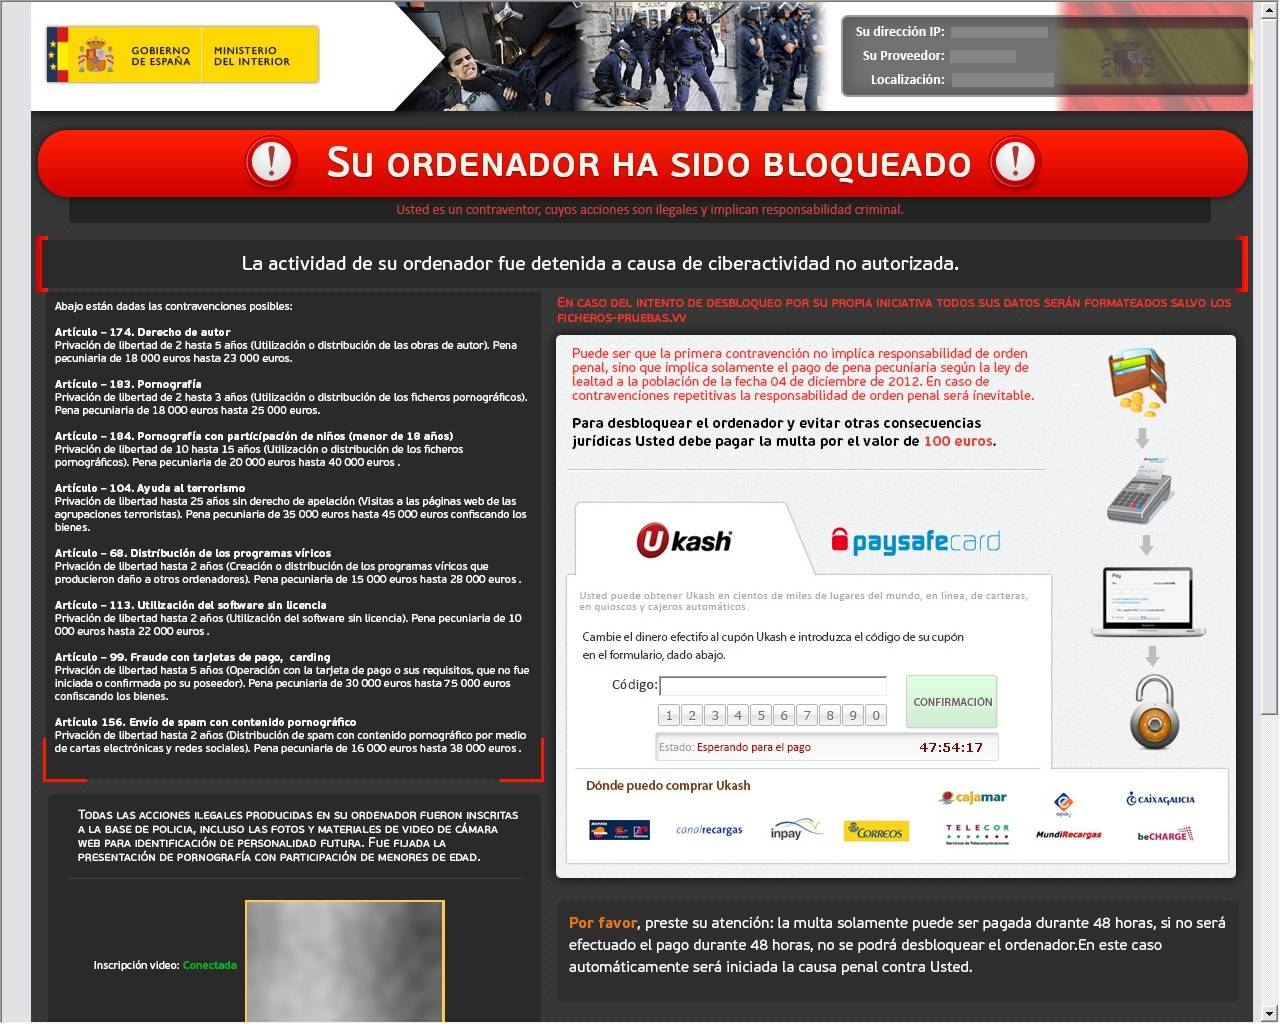
\includegraphics[width=0.75\linewidth]{images/ransomware} 

}

\caption{Ransomware (Malware).}\label{fig:unnamed-chunk-14}
\end{figure}

\hypertarget{spyware-o-software-espuxeda}{%
\section{Spyware o software espía}\label{spyware-o-software-espuxeda}}

El spyware es un otro tipo de malware que se mantiene oculto mientras mientras recopila información en secreto, que después transmite a una entidad externa sin el conocimiento o el consentimiento del propietario del dispositivo \citep{AVAST-spyware}.

Puede supervisar y copiar todo lo que escribes, cargas, descargas y almacena. Algunas cepas de spyware también son capaces de activar cámaras y micrófonos sin que te des cuenta.

Un spyware típico se auto instala en el sistema afectado de forma que se ejecuta cada vez que se pone en marcha el ordenador (utilizando CPU y memoria RAM, reduciendo la estabilidad del ordenador), y funciona todo el tiempo, controlando el uso que se hace de Internet e incluso algunos muestran anuncios relacionados.

Sin embargo, a diferencia de los virus, no se intenta replicar en otros ordenadores, por lo que funciona como un parásito.

El spyware tiene diferentes vías de entrada a nuestros equipos, muy parecidas a los virus y gusanos:

\begin{itemize}
\item
  Descarga de contenidos mediante redes de compartición P2P u otras fuentes poco fiables.
\item
  Apertura de algún fichero adjunto en un correo electrónico.
\item
  Visitar a una web maliciosa, al pulsar sobre alguna dirección acortada que se publican en redes sociales y que en verdad no sabemos a qué páginas web nos llevarán.
\end{itemize}

\hypertarget{phishing-pharming-typosquatting}{%
\section{Phishing / pharming / typosquatting}\label{phishing-pharming-typosquatting}}

El término Phishing es utilizado para referirse a uno de los métodos más utilizados por delincuentes cibernéticos para estafar y obtener información confidencial de forma fraudulenta como puede ser una contraseña o información detallada sobre tarjetas de crédito u otra información bancaria de la víctima \citep{INFOSPY-phishing}.

El estafador, conocido como phisher, se vale de técnicas de \href{https://es.wikipedia.org/wiki/Ingeniería_social_(seguridad_informática)}{ingeniería social}, haciéndose pasar por una persona o empresa de confianza en una aparente comunicación oficial electrónica, por lo general un correo electrónico, redes sociales, SMS, etc., a raíz de un malware o incluso utilizando también llamadas telefónicas.

Los métodos de phishing más usados por lo ciberdelincuentes:

\begin{itemize}
\item
  Correos electrónicos de carácter corporativo.
\item
  Mensajería instantánea.
\item
  Redes sociales.
\item
  Webs corporativas (Bancos, pasarelas de pago, tiendas online, etc.)
\item
  SMS.
\end{itemize}

Para poder detectar si estas siendo víctima de uno de estos fraudes debes estar atento a lo siguiente:

\begin{itemize}
\item
  La dirección web o URL: Fíjate muy bien en la URL a la que te remite el enlace que te envían. Insistir en que hay que fijarse muy bien porque en algunas ocasiones las diferencias son inapreciables y se centran incluso en caracteres que se copian o se alteran (una l minúscula por una i mayúscula; un punto situado en un lugar poco visible y otras estrategias).
\item
  Ortografía: Forma en la que está redactado el mensaje. Los ciberatacantes en algunos casos no tienen tu misma nacionalidad ni hablan tu mismalengua y, en muchas ocasiones traducen los textos automáticamente y contienen faltas de ortografía, errores gramaticales o un tratamiento o forma de dirigirse a ti que ninguna comunicación oficial de tu banco, organismos o empresas contendría.
\item
  Cuidado con el remitente y lo que solicitan: Correo electrónico de tu banco, de la Agencia Tributaria, de Amazon u otra empresa. Lo primero que debes mirar es el remitente y comprobar que esa dirección es la que está vinculada a esos servicios. De la misma manera, si el correo te ha llegado a la carpeta de spam ya es un signo inequívoco de que el remitente es sospechoso. ¿Qué te piden en el correo? Ten muy presente que los bancos y las empresas u organismos no reclaman jamás que introduzcas tus datos personales o que los reingreses en una web para reactivar tu cuenta. No lo reclaman jamás.
\item
  Desconfía de los cupones promocionales y las encuestas: Esta modalidad de phishing ha sido una de las que más éxito ha tenido en los últimos años y ha afectado a todas las grandes marcas. Existen ejemplos de phishing a Mercadona, Ikea, a El Corte Inglés, a Zara, a Lidl\ldots{} Y todo a través de cupones promocionales en los que te prometen una compra o un vale descuento a cambio de que accedas a un enlace y rellenes tus datos personales.
\item
  Descarga archivos adjuntos: Salvo que hayas comprobado todos los pasos anteriores y estés completamente seguro de la identidad del remitente, así como del objeto del mensaje, no descargues documentos adjuntos sin antes pasarlos por un buen antivirus.
\item
  Usa el sentido común y desconfía siempre: Este consejo es válido para detectar el phishing o cualquier otra amenaza en Internet. ¿Quién va a regalar gafas Ray-Ban o a venderlas un 75\% por debajo de su precio?.
\end{itemize}

\begin{figure}

{\centering 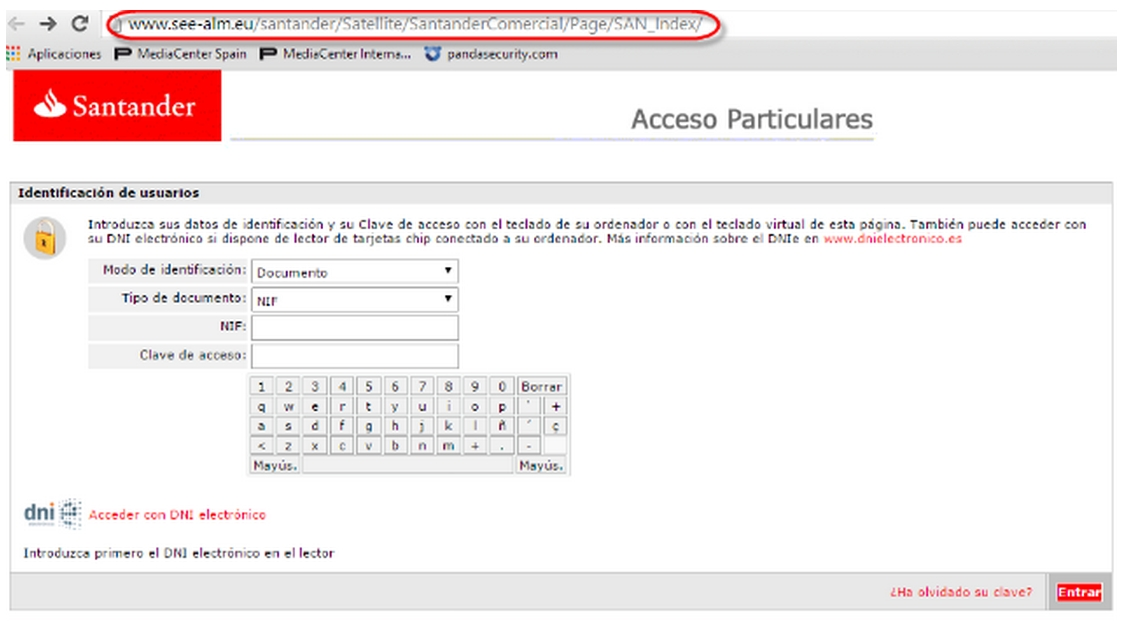
\includegraphics[width=1\linewidth]{images/phishing} 

}

\caption{Phishing banco Santander.}\label{fig:unnamed-chunk-15}
\end{figure}

El Pharming es la explotación de una vulnerabilidad en el software de los servidores DNS (Domain Name System) o en el de los equipos de los propios usuarios, que permite a un atacante redirigir un nombre de dominio (domain name) a otra máquina distinta. De esta forma, un usuario que introduzca un determinado nombre de dominio que haya sido redirigido, accederá en su explorador de internet a la página web que el atacante haya especificado para ese nombre de dominio \citep{WIKI-pharming}.

El Typosquatting, también conocido como URL hijacking, sting site, o fake URL. Está basada en los errores tipográficos cometidos por usuarios de internet cuando introducen la dirección de un sitio web en un navegador. Cuando esto sucede la dirección puede llevarlos a un sitio alternativo propiedad de un cybersquatter \citep{WIKI-typosquatting}.

\begin{itemize}
\tightlist
\item
  Ejemplo: \url{https://wikiepdia.org}
\end{itemize}

\hypertarget{vishing}{%
\section{Vishing}\label{vishing}}

vishing

\hypertarget{smishing}{%
\section{Smishing}\label{smishing}}

smishing

\hypertarget{spam-o-correo-malicioso}{%
\section{Spam o correo malicioso}\label{spam-o-correo-malicioso}}

Los términos spam o correo malicioso hacen referencia a los mensajes no solicitados, no deseados o con remitente no conocido (correo anónimo), habitualmente de tipo publicitario, generalmente son enviados en grandes cantidades (incluso masivas) que perjudican de alguna o varias maneras al receptor \citep{WIKI-spam}.

Su finalidad suele ser con motivos comerciales, pero también pueden contener enlaces peligros como el Phishing, solicitar datos sensibles o contener descargas que sean un riesgo para nuestra privacidad y seguridad:

\begin{itemize}
\item
  E-Mails Spam con fines comerciales
\item
  Envíos masivos / Avisos de virus
\item
  E-Mails con ofertas o regalos
\item
  Correos Phishing
\end{itemize}

Si recibes un email de carácter sospechoso, no lo abras y márcalo directamente como spam, para que así tu gestor de correos lo identifique para los sucesivos.

\hypertarget{toolbars}{%
\section{Toolbars}\label{toolbars}}

Las Toolbars son barras de herramientas que aparecen en la parte superior de los navegadores. Generalmente sirven para tener enlaces más rápidos a servicios, por ejemplo Windows Live Toolbars da acceso al correo y búsqueda entre otras funcionalidades. Regularmente los navegadores tienen las suyas propias.

Pero puede ocurrir que a través de una instalación de software, normalmente gratuito puedan ser instaladas. Debes tener en cuenta que algunas de estas son muy molestas y en algunos casos pueden llegar a bombardearte con publicidad no deseada y que además en ocasiones llegan a ser muy difíciles de eliminar. Aunque cada vez son memos frecuentes.

\begin{figure}

{\centering 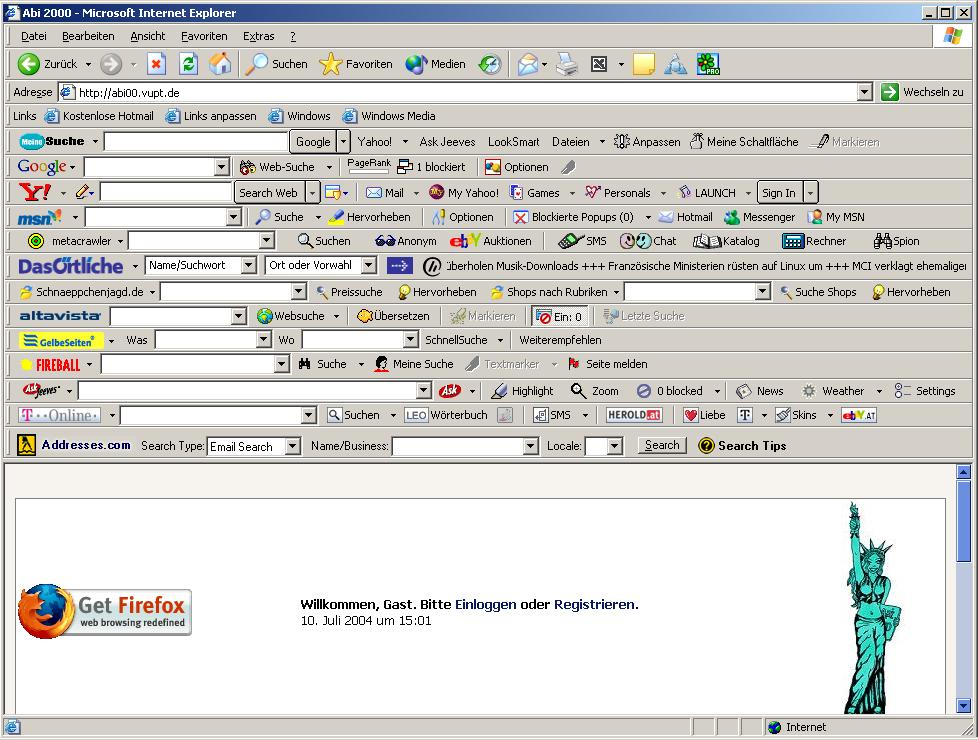
\includegraphics[width=0.75\linewidth]{images/toolbar} 

}

\caption{Toolbar.}\label{fig:unnamed-chunk-16}
\end{figure}

Normalmente, se instalan como un añadido al instalar aplicaciones gratuitas en el ordenador. Si no tienes cuidado durante el proceso de instalación y pulsamos siempre ``Siguiente-Siguiente-Siguiente'' las toolbars acaban en nuestro navegador. Para evitarlo no debes instalar una aplicación dando a ``Siguiente-Siguiente-Siguiente'' sin leer lo que nos están indicando. Para evitar este supuesto, recuerda que lo mejor es descargar programas solo de las webs oficiales.

En el caso de haber instalado alguna toolbars por descuido existen algunas herramientas para desinstalarlas fácilmente, entre ellas esta \href{https://es.malwarebytes.com/adwcleaner/}{Malwarebytes}.

\hypertarget{usurpaciuxf3n-o-robo-de-identidad}{%
\section{Usurpación o robo de identidad}\label{usurpaciuxf3n-o-robo-de-identidad}}

El robo de identidad o usurpación de identidad es la apropiación de la identidad de una persona: hacerse pasar por esa persona, asumir su identidad ante otras personas en público o en privado, en general para acceder a ciertos recursos o la obtención de créditos y otros beneficios en nombre de esa persona. Esto que sucede en el mundo analógico también ocurre en el mundo digital \citep{WIKI-usurpacion}.

La manera que tienen los ciberdelincuentes de usurpar la identidad suele ser a través de los siguientes:

\begin{itemize}
\item
  Robo masivo de cuentas de email por medio de métodos de hacking.
\item
  Por medio de Phishing.
\item
  Dejando tú cuenta abierta en sitios públicos.
\item
  Usando Wi-Fi de terceros creadas para ese fin.
\end{itemize}

La usurpación de identidad permite a los delincuentes hacerse con información personal de sus víctimas, para luego con ella interceptar aún más datos de otros perfiles, a quienes engañan con el fin de extorsionar u obtener lucro económico e incluso a veces realizar actividades delictivas.
En caso de ser víctima de esta amenaza debes tener en cuenta lo siguiente:

\begin{itemize}
\item
  Guarda los mensajes de texto e emails que recibas.
\item
  Haz capturas de pantalla.
\item
  Revisa todas tus redes sociales.
\item
  Avisa a tus contactos sobre el perfil falso.
\item
  Infórmalo dentro de la aplicación.
\item
  Si es de carácter grave denúncialo a las autoridades.
\item
  Si es posible cancela cuenta.
\end{itemize}

\hypertarget{estafas-en-compras-online-y-otros-engauxf1os}{%
\section{Estafas en compras online y otros engaños}\label{estafas-en-compras-online-y-otros-engauxf1os}}

Pago del envio por una venta de segunda mano, etc

\hypertarget{vulnerabilidades}{%
\section{Vulnerabilidades}\label{vulnerabilidades}}

Una vulnerabilidad en términos de informática es una debilidad o fallo en un sistema de información que pone en riesgo la seguridad de la información pudiendo permitir que un atacante pueda comprometer la integridad, disponibilidad o confidencialidad de la misma. Estas vulnerabilidades pueden tener distintos orígenes como por ejemplo: fallos de diseño, errores de configuración o carencias de procedimientos \citep{INCI-vulnerabilidad}.

Los fallos de vulnerabilidad les corresponde corregirlos a las terceras partes implicadas lo a veces con lleva la dificultad de que escapan a nuestro control. Pero para protegernos de tales, debemos tener actualizados todos nuestros sistemas y software.

Un ejemplo de vulnerabilidad muy conocido fuero el \href{https://es.wikipedia.org/wiki/Meltdown_(vulnerabilidad)}{Meltdown} y \href{https://es.wikipedia.org/wiki/Spectre_(vulnerabilidad)}{Spectre}, relacionadas con los procesadores informáticos, que existen desde mediados de los noventa, pero que han sido descubiertas solamente ahora.

\hypertarget{cryptojacking}{%
\section{Cryptojacking}\label{cryptojacking}}

El cryptojacking, también llamado minería de criptomonedas malicioso, consiste en un tipo de software fraudulento que se oculta en un ordenador o en un dispositivo móvil, y utiliza los recursos de la máquina para extraer diversas formas de monedas digitales conocidas como \href{https://es.wikipedia.org/wiki/Criptomoneda}{criptomonedas}. Hay que aclarar que no está tan focalizado en el robo directo de estas, sino, que se centra en el robo o secuestro de dispositivos de terceros con el fin de utilizarlos para minar estas criptomonedas, y a los que se le conocen también como dispositivos zombies \citep{cryptojacking}.

Se trata de una amenaza reciente que se hace con el control del navegadores web, y de este modo, comprometen todo tipo de dispositivos, desde ordenadores de escritorio y portátiles hasta teléfonos inteligentes e incluso servidores de red.

Existen recursos y herramientas para saber si estamos siendo víctimas de cryptojacking:

\begin{itemize}
\item
  Te puede pasar que el ordenador se recaliente, que empiecen a sonar los ventiladores de pronto y se mantengan encendidos por más tiempo de lo que consideras normal.
\item
  El sistema operativo se pondrá lento, incluso se puede llegar a colgar el navegador o todo el sistema constantemente.
\item
  Comprueb el administrador de tareas en Windows, o el Monitor de actividad en MacOS. Fíjate en los procesos que estén ocupando el mayor porcentaje de CPU. En circunstancias normales un solo proceso no debe pasar de 10\%, rara vez sobrepasan el 20\% al menos que se trate de software muy complejo como el de edición de vídeo, juegos, o el mismo sistema actualizando. Pero que te aparezca el navegador en números absurdos como 70-90 y hasta 100\% es una alarma clara.
\end{itemize}

Las vías de contagios son las mismas que la mayoría de malware tales como los virus, gusanos, troyanos, spyware y demás. Por lo que puedes verlo en dichos apartados de esta misma unidad. Aunque en la mayoría de los casos te llega a través de una web, haciendo uso del navegador por lo que existen webs y plugin que comprueban si estas siendo víctima de este ciberdelito y algunas de estas son:

\begin{itemize}
\item
  \href{https://github.com/fhstp/CoinEater}{CoinEater}
\item
  \href{https://github.com/xd4rker/MinerBlock}{Minerblock}
\item
  \href{https://notmining.es}{Not mining}
\end{itemize}

\hypertarget{plugins-maliciosos}{%
\section{Plugins maliciosos}\label{plugins-maliciosos}}

En primer lugar, es importante tener claro qué es un plugin. Así pues, se trata de un software o aplicación que actúa como complemento para ampliar las funcionalidades del programa principal al que complementa. Dicho esto, algunos ciberdelicuentes usan esta funcionalidad para sus actividades delictivas, como espiar o recopilar datos sensibles e incluso el robo de criptomonedas. \citep{WIKI-plugin}.

Instalar un plugin suele ser una acción muy sencilla, y te puede servir para finalidades muy diversas, un claro ejemplo ello, es el plugin de \href{https://drive.googleblog.com/2012/12/introducing-save-to-drive-extension.html}{Google drive} o \href{https://getadblock.com/}{Adblock} para el bloqueo de publicidad, etc. Es por esto que debes tener siempre algunas consideraciones, como verás a continuación.

Sin embargo, a pesar de ser programas muy útiles que la inmensa mayoría utiliza, no todos son conscientes del riesgo que conlleva el simple hecho de instalar un plugin. El problema suele venir por no tener actualizado un buen sistema de seguridad.

A veces, el simple hecho de que el plugin este disponible no significa garantía ninguna. Tanto es así que aquí podemos ver uno de los que recientemente ha sido retirado de WordPress hasta en cuatro ocasiones. Un programa capaz de recopilar datos de los navegantes con el correspondiente riesgo a nivel de Reglamento General de Protección de Datos que esto conlleva, así como de publicar entradas no deseadas y prácticas de spam. De otra lado Google esta continuamente retirando plugins maliciosos de su plataforma.

Los puntos más importantes a tener en cuenta a la hora de protegernos son:

\begin{itemize}
\item
  Infórmate del desarrollo del plugin así como posibles variaciones.
\item
  No descarges plugins sospechosos.
\item
  Utiliza preferiblemente aquellos plugins de referencia, con fama y garantía reconocidas.
\end{itemize}

\hypertarget{sim-swaping}{%
\section{SIM Swaping}\label{sim-swaping}}

El SIM swapping,es la técnica que usan últimamente los ladrones digitales que se basa en duplicar la tarjeta SIM del móvil de sus víctimas. Así, pueden acceder a toda su información personal y, sobre todo, pueden usarlas en la verificación a través de un SMS por medio del móvil que suelen pedir los bancos cuando se opera a través de Internet y algunas otras plataformas online.

Por ello, aunque la mayoría de las apps de los bancos son muy seguras, con protocolos complejos para las claves de acceso, cifrado de las comunicaciones y teclados virtuales, los timadores digitales son capaces de saltarse la seguridad por medio de una técnica llamada \href{https://es.wikipedia.org/wiki/Ingeniería_social_(seguridad_informática)}{ingeniería social}, que consiste en el engaño a través de técnicas de persuasión y manipulación psicológica. Sin embargo, en lugar de timar directamente a las víctimas, el SIM swapping se consigue por medio de un engaño a los dependientes de las tiendas de telefonía.

Por lo tanto, una vez que el ciberdelicuente se hace con tus credenciales del tipo que sea, tales como contraseñas bancarias o de perfiles sociales, como Facebook, Instagram, etc o cualquier otra credencial privada, no va a tener problemas para obtener el SMS de verificación.

Cabe destacar que cuando se es víctima de este asalto digital, al obtener la duplicación de la SIM por parte del atacante, tu tarjeta queda sin uso, por lo tanto pierdes la cobertura de llamadas y la conexión de internet \citep{PANDA-sim}.

Por lo tanto, es importante que sigas estas recomendaciones para no ser víctimas del SIM Swapping:

\begin{itemize}
\item
  Utiliza una contraseña adicional o \href{https://www.osi.es/es/actualidad/blog/2019/02/27/el-factor-de-autenticacion-doble-y-multiple}{doble autentificación}: reconocimiento facial, por voz, PIN adicional, \href{https://play.google.com/store/apps/details?id=com.google.android.apps.authenticator2\&hl=es\&gl=US}{Google authenticator}, etc.
\item
  No compartas demasiada información en Internet. Cuantos más datos haya sobre ti en la web, más fácil será para los malos chantajearte, timarte o conseguir otras cosas tuyas, como contraseñas, cuentas bancarias, etc.
\item
  No almacenes todo en tu móvil, no es una caja fuerte. Es un dispositivo electrónico que no es 100\% seguro.
\item
  Exige a tu operador móvil que refuerce sus sistemas de seguridad cuando se trate de operaciones en tu nombre.
\item
  Los mensajes a través de aplicaciones de mensajería tipo WhatsApp, Telegram, Line, etc. son más seguros que los SMS, ya que están encriptados y éstos últimos no, haciéndolos más susceptibles.
\item
  No vincules tus cuentas bancarias a tu cuenta o teléfono.
\item
  No le des nunca a nadie tu código PIN. ¡Nunca!.
\item
  Instala un antivirus o solución de seguridad para evitar que puedan robar o acceder a tus datos personales.
\end{itemize}

Qué hacer en caso de que ya te hayan robado tu dispositivo móvil:

\begin{itemize}
\item
  Pide a tu operadora que bloquee el IMEI de tu teléfono.
\item
  Búscalo con el localizador para \href{https://myaccount.google.com/intro/find-your-phone?hl=es-ES}{android} para \href{https://www.apple.com/es/icloud/find-my/}{apple}.
\item
  Anula la SIM y pide duplicado de la misma.
\item
  Cambia todas tus contraseñas. ¡Todas!.
\item
  Denúncialo a la Policía.
\item
  Denúncialo a tu operadora
\item
  Avisa a tus contactos. Sí, a todos.
\item
  Bloquea el dispositivo y borra el contenido que puedas de forma remota.
\item
  Comprueba tu cuenta bancaria y ponte en contacto con tu banco.
\end{itemize}

Ve este \href{https://www.youtube.com/watch?v=fIaodow_nxw}{video} del \href{https://www.incibe.es/}{Instituto nacional de Ciberseguridad}

\hypertarget{shoulder-surfing}{%
\section{Shoulder surfing}\label{shoulder-surfing}}

Shoulder

\hypertarget{ciberacoso}{%
\section{Ciberacoso}\label{ciberacoso}}

acoso

\hypertarget{ciberextorsiuxf3n}{%
\section{Ciberextorsión}\label{ciberextorsiuxf3n}}

que es la ciberextorsión

\hypertarget{otros-conceptos-relacionados}{%
\chapter{Otros conceptos relacionados}\label{otros-conceptos-relacionados}}

\hypertarget{otros-conceptos-que-te-pueden-ayudar}{%
\section{Otros conceptos que te pueden ayudar}\label{otros-conceptos-que-te-pueden-ayudar}}

En esta última unidad podrás ver otros aspectos relacionados con la privacidad y seguridad en internet que también te pueden ayudar a abordar todos estos temas.

\hypertarget{metadatos}{%
\section{Metadatos}\label{metadatos}}

Los metadatos pueden ser descritos de varias formas posibles, pero de forma resumida son un conjunto de datos que proporciona información de un recurso. Datos como pueden ser un archivo de imagen o un documento de texto, siendo algunos de éstos metadatos la fecha de creación, la de última modificación o la resolución en el caso de una imagen \citep{WIKI-meta}.

La función principal de los metadatos es la de ampliar con información adicional la contenida en el recurso del que forman parte con el fin de mejorar la calidad y efectividad de las búsquedas realizadas, no solo a la hora de realizar una búsqueda de un archivo perdido en nuestro sistema operativo, sino que esto afecta incluso al posicionamiento web.

En ciertas ocasiones éstos datos pueden provocar problemas, algunos de ellos de seguridad como puede ocurrir por ejemplo por alguno de los dos motivos siguientes:

\begin{itemize}
\item
  Suele ocurrir que algunas cámaras fotográficas incluyan las coordenadas geográficas desde las que se realiza la fotografía entre los metadatos en los archivos de imágenes, pudiéndose localizar la posición en la que la imagen fue tomada.
\item
  Puede determinarse la versión del software con la que fue guardado un archivo, por lo que si trabajas en una empresa y no tienes la licencia de dicho programa, los metadatos pueden generarte problemas.
\end{itemize}

\hypertarget{huella-digital-o-reputaciuxf3n-online}{%
\section{Huella digital o reputación online}\label{huella-digital-o-reputaciuxf3n-online}}

La huella digital o reputación online es la fama o prestigio que una persona o una empresa tiene en el mundo digital. Realmente la reputación digital no difiere mucho de la reputación tradicional, ya que en cierto modo ambas están conectadas, por lo que deben ser coherentes la una con la otra.

Cabe destacar que la variante digital ha tomado gran importancia, ya que cuando una persona o compañía quiere saber de ti, uno de los mecanismos que va a utilizar es buscarte en internet, y es, en este punto donde radica la importancia de contar con una buena reputación online \citep{huella-digital}.

En este sentido es importante en un primer momento, conocer si tu huella digital goza de una buena salud y para ello lo más recomendable es que hagas un ejercicio de búsqueda, para ver si los resultados que obtienes son buenos. Puedes usar algunas de la siguientes herramientas para este propósito:

\begin{itemize}
\item
  Buscar directamente en google o otros buscadores. Puedes apoyarte en las \href{https://support.google.com/websearch/answer/2466433?hl=es}{búsquedas avanzadas de google}.
\item
  Crear alertas de \href{https://www.google.es/alerts}{Google alert}. Este rcurso también te servira para estar al día de lo que se publica sobre ti.
\item
  \href{https://www.hootsuite.com/}{Hootsuite}. Esta herramienta te buscará entre las principales redes sociales, como Facebook, twitter, etc. es usada en su mayoría en el mundo corporativo.
\end{itemize}

Si los resultados obtenidos no son de tu agrado, algunas plataformas te permiten solicita la eliminación de dicho contenido o simplemente puedes gestionar tu esa información desde la propia plataforma.

Crear una buena huella digital requiere de tiempo y debes ser cuidadoso con la manera en que interactuas en la red. Existen decálogos que te guían para crear una excelente reputación online, así como videos tutoriales y herramientas para llevarlo a cabo. Nos obstante aquí tienes las mejores recomendaciones para cuando quieras compartir, comentar, valorar o opinar en cualquiera de los medios sociales como Facebook, Instagram o cualquier otra, hacer una reseña en google o participar en algún foro \citep{decalogo-digital}.

\begin{itemize}
\item
  Presencia y actualización sistemática.
\item
  Cuidar la imagen mostrando transparencia.
\item
  Aportar contenido de calidad.
\item
  Respetar siempre la opinión ajena.
\item
  Identificar los canales apropiados con los que interactuar.
\item
  Tener en cuenta las reglas de urbanidad digital, esto consiste en una redacción cuidada y usos de negritas o enlaces de interés.
\item
  Diferenciar entre lo público y lo privado.
\end{itemize}

Estas últimas puedes tenerlas en cuenta si quieres llevar tu huella digital a un nivel más profesional.

\begin{itemize}
\item
  Disponer de un blog personal.
\item
  Mantener una actitud en la red activa.
\item
  Permanecer atento a las nuevas redes y formas de difusión.
\end{itemize}

\hypertarget{eliminar-el-historial-de-busquedas}{%
\section{Eliminar el historial de busquedas}\label{eliminar-el-historial-de-busquedas}}

Cualquier navegador, salvo que usemos una navegación privada, almacena un registro de las páginas que hemos visitado, una información que podemos borrar si queremos o conservar en el caso de querer localizar más tarde alguna página que no recordemos. Es muy útil en este segundo caso, pero puede llegar a ser embarazoso si no queremos que nadie pueda ver las webs que hemos visitado.

Cada navegador ofrece la posibilidad de borrar toda esta información y para ello accederemos desde los menús de estos. Cada navegador tiene una forma diferente de realizar este borrado, aunque normalmente suele estar en la opción/pestaña herramientas. No obstante el siguiente enlace te llevará a la web del antivirus \href{https://www.avg.com/es/signal/how-to-clear-your-browsing-and-search-history}{AVG}, desde donde te enlazará a los diferentes tutoriales de cómo borrar el historial de navegación y de búsquedas de los navegadores más populares, como Google Chrome, Firefox o Microsoft Edge entre otros.

\hypertarget{constastar-la-informaciuxf3n}{%
\section{Constastar la información}\label{constastar-la-informaciuxf3n}}

Contrastar es sacar la información más relevante de los diferentes lugares en los que la encontramos, ya que es una idea principal de aquello que necesitamos comprender o aplicar. Hoy en día la información en más rápida de encontrar, por lo cual hay que saberla escoger, porque en muchos casos son cosas irrelevantes que las personas ponen solo para confundir o simplemente por falta de conocimiento o criterio.

Al contrastar información debes hacer un análisis de todas aquellas fuentes de información que encuentras, ya que los resultados de búsquedas en los navegadores es muy abundante y la información a veces es efímera y puede llegar a no estar totalmente actualizada, con lo que eso conlleva.

No debemos conformarnos con dar por buena la primera versión de una información en Internet, empobrece nuestra experiencia como usuarios, nos perjudica a nosotros los lectores. Por ello hay que tener presente el compromiso ético, por mucho que las prisas sean las que mandes en algunas ocasiones, siempre debemos cuidar nuestra ética al trabajar y contrastar muy bien toda información y fuente \citep{contrastar-informacion}.

\hypertarget{otras-utilidades-interesantes}{%
\section{Otras utilidades interesantes}\label{otras-utilidades-interesantes}}

Aparte de todo lo visto en el manual existen muchas otras herramientas para ayudarnos a salvaguardar nuestra privacidad y seguridad en la red, algunas de estas son:

\begin{itemize}
\item
  Emails temporales: \href{https://temp-mail.org/es/}{Temporay email}. Si solo necesitas regístrarte en una web para un recurso puntual, como por ejemplo descargarte un eBook, puedes hacer uso de este servicio. Y si usas el navegador Firefox, podrás tener este mismo servicio integrado en el propio navegador con solo la instalación de un plugin \href{https://relay.firefox.com}{Relay firefox}.
\item
  Escaneo de URLs maliciosas: \href{https://urlscan.io/}{UrlScan}. Esta plataforma detecta las direcciones webs fraudulentas.
\item
  Comprobar y mejorar tu privacidad y seguridad en internet: \href{https://securitycheckli.st/}{Lista de verificación de seguridad}. Esta web esta en inglés pero abarca un amplio espectro de herramientas y recursos diseñados para mejorar tu privacidad, seguridad y protección online y siempre dispones del traductor en línea de google.
\item
  Eliminar cuentas en Redes Sociales: \href{https://www.deseat.me/}{Deseat}. Con esta plataforma podrás tener instantáneamente una lista de todas tus cuentas y eliminar las que no estés usando o las que te apetezcan.
\item
  Números de teléfono de usar y tirar: \href{https://hushed.com}{Hushed}. Se trata de un servicio premiun pero de coste muy económico. Solo es cuestión de ver si te compensa.
\item
  Nombres y direcciones desechables: \href{https://www.fakenamegenerator.com}{Generador de nombres falsos}. Como en el caso de los emails temporales este servicio puede ser un buen recurso.
\end{itemize}

\hypertarget{entidades-e-instuciones-de-ayuda-al-ciudadano}{%
\section{Entidades e instuciones de ayuda al ciudadano}\label{entidades-e-instuciones-de-ayuda-al-ciudadano}}

\textbf{INSTITUTO NACIONAL DE CIBERSEGURIDAD} \href{https://www.incibe.es/}{INCIBE}

El Instituto Nacional de Ciberseguridad de España (INCIBE), es una sociedad dependiente del Ministerio de Economía y Empresa a través de la Secretaría de Estado para el Avance Digital y consolidada como entidad de referencia para el desarrollo de la ciberseguridad y de la confianza digital de ciudadanos, red académica y de investigación, profesionales, empresas y especialmente para sectores estratégicos.

La misión de INCIBE es por tanto reforzar la ciberseguridad, la confianza y la protección de la información y privacidad en los servicios de la Sociedad de la Información, aportando valor a ciudadanos, empresas, Administración, red académica y de investigación española, sector de las tecnologías de la información y las comunicaciones y sectores estratégicos en general. Aunándolo es estas tres siguientes líneas de actuación:

\begin{itemize}
\item
  Al internauta.
\item
  Al menor.
\item
  A la empresa.
\end{itemize}

Informan entre otros sobre:

\begin{itemize}
\item
  Protección de redes, equipos y sistemas.
\item
  Cumplimiento de obligaciones relativas a la seguridad de la información.
\item
  Diferentes tipos de incidentes de seguridad.
\item
  Seguridad en las conexiones y redes wifi.
\item
  Configuración de la privacidad en dispositivos y servicios de internet.
\item
  Situaciones de infección por virus.
\item
  Contenidos inadecuados para menores y comunidades peligrosas en línea.
\item
  Ciberacoso escolar.
\item
  Controles parentales.
\end{itemize}

Dispone de un teléfono gratuito 017.

\textbf{OFICINA DE SEGURIDAD DEL INTERNAUTA} \href{https://www.osi.es/es}{OSI}

Hola

\textbf{AGENCIA ESPAÑOLA DE PROTECCIÓN DE DATOS} \href{https://www.aepd.es/es}{AEPD}

Hola

En caso de tratarse de menores

\textbf{PANTALLAS AMIGAS} \href{https://www.pantallasamigas.net/}{Pantallasamigas.net}

Para menores

\textbf{INTERNET SEGURA PARA NIÑOS} \href{https://www.is4k.es/}{is4k}

Para niños

  \bibliography{book.bib,article.bib,manual.bib}

\end{document}
